% ============================================================================
%  DT7429 Layer 2 Managed Switch -- User Guide
%  Chapter: VLAN Configuration
%  Style: Cisco-style technical manual
%
%  Compile with XeLaTeX
% ============================================================================

\documentclass[11pt,letterpaper]{report}

% ---------------------------------------------------------------------------
% Packages
% ---------------------------------------------------------------------------
\usepackage[margin=1in,headheight=14pt]{geometry}
\usepackage{fancyhdr}
\usepackage{titlesec}
\usepackage{xcolor}
\usepackage{tcolorbox}
\tcbuselibrary{skins,breakable}
\usepackage{longtable}
\usepackage{array}
\usepackage{booktabs}
\usepackage{listings}
\usepackage{enumitem}
\usepackage{hyperref}
\usepackage{graphicx}
\usepackage{caption}
\usepackage{parskip}
\usepackage{fontawesome5}

% ---------------------------------------------------------------------------
% Persian / Bilingual support
% Compile using XeLaTeX
% ---------------------------------------------------------------------------
\usepackage{xepersian}

% Replace Vazirmatn with an installed Persian font if necessary.
\settextfont{Vazirmatn}
\setlatintextfont{Latin Modern Roman}
\setmonofont{DejaVu Sans Mono}

% ---------------------------------------------------------------------------
% Colors (Cisco-esque palette)
% ---------------------------------------------------------------------------
\definecolor{ciscoblue}{RGB}{0,84,157}
\definecolor{ciscodarkblue}{RGB}{0,50,94}
\definecolor{ciscolightgray}{RGB}{245,247,250}
\definecolor{cisconote}{RGB}{230,242,255}
\definecolor{ciscowarn}{RGB}{255,243,224}
\definecolor{ciscocaution}{RGB}{255,235,235}
\definecolor{codebg}{RGB}{40,44,52}
\definecolor{codefg}{RGB}{220,223,228}
\definecolor{codegreen}{RGB}{152,195,121}
\definecolor{codegray}{RGB}{130,137,151}
\definecolor{codeblue}{RGB}{97,175,239}

% ---------------------------------------------------------------------------
% Section title styling
% ---------------------------------------------------------------------------
\titleformat{\chapter}[display]
{\normalfont\huge\bfseries\color{ciscoblue}}
{\Large\color{ciscodarkblue}\lr{Chapter \thechapter}}
{10pt}{\Huge}
\titlespacing*{\chapter}{0pt}{0pt}{30pt}

\titleformat{\section}
{\normalfont\Large\bfseries\color{ciscoblue}}
{\thesection}{10pt}{}

\titleformat{\subsection}
{\normalfont\large\bfseries\color{ciscodarkblue}}
{\thesubsection}{8pt}{}

\titleformat{\subsubsection}
{\normalfont\normalsize\bfseries\color{ciscodarkblue}}
{\thesubsubsection}{6pt}{}

% ---------------------------------------------------------------------------
% Header / Footer
% ---------------------------------------------------------------------------
\pagestyle{fancy}
\fancyhf{}
\renewcommand{\headrulewidth}{0.6pt}
\renewcommand{\footrulewidth}{0.4pt}

\fancyhead[L]{%
	\small\color{ciscodarkblue}
	\lr{\textbf{DT7429 Layer 2 Managed Switch}}%
}

\fancyhead[R]{%
	\small\color{ciscodarkblue}
	\lr{User Guide}%
}

\fancyfoot[L]{%
	\small\color{gray}
	\lr{Doc: VAF-11111111}%
}

\fancyfoot[R]{%
	\small\color{gray}\thepage%
}

% ---------------------------------------------------------------------------
% Code / CLI listing style
% ---------------------------------------------------------------------------
\lstdefinelanguage{ciscoios}{
	morekeywords={
		configure,terminal,interface,vlan,name,exit,end,show,switchport,
		mode,access,trunk,allowed,add,remove,native,voice,private,mapping,
		host,promiscuous,isolated,community,host-association,range,no,clear,
		mac,address,table,dynamic
	},
	sensitive=false,
	morecomment=[l]{!},
}

\lstset{
	backgroundcolor=\color{codebg},
	basicstyle=\ttfamily\footnotesize\color{codefg},
	keywordstyle=\color{codeblue}\bfseries,
	commentstyle=\color{codegray}\itshape,
	stringstyle=\color{codegreen},
	breaklines=true,
	breakatwhitespace=false,
	frame=single,
	framerule=0pt,
	rulecolor=\color{codebg},
	xleftmargin=8pt,
	xrightmargin=8pt,
	framexleftmargin=8pt,
	framexrightmargin=8pt,
	framextopmargin=6pt,
	framexbottommargin=6pt,
	showstringspaces=false,
	columns=fullflexible,
	language=ciscoios,
	literate={\$}{{\textcolor{codegreen}{\$}}}1
}

% ---------------------------------------------------------------------------
% Callout boxes: Note / Caution / Tip
% ---------------------------------------------------------------------------
\newtcolorbox{noticebox}[2][]{
	breakable,
	enhanced,
	colback=#2!12,
	colframe=#2!70!black,
	boxrule=0.6pt,
	left=8pt,
	right=8pt,
	top=5pt,
	bottom=5pt,
	arc=1.5pt,
	#1
}

\newenvironment{notebox}[1]{%
	\begin{noticebox}[title={\textbf{\faInfoCircle\ #1}}]{cisconote}
	}{%
	\end{noticebox}
}

\newenvironment{cautionbox}[1]{%
	\begin{noticebox}[title={\textbf{\faExclamationTriangle\ #1}}]{ciscocaution}
	}{%
	\end{noticebox}
}

\newenvironment{tipbox}[1]{%
	\begin{noticebox}[title={\textbf{\faLightbulb\ #1}}]{ciscowarn}
	}{%
	\end{noticebox}
}

% ---------------------------------------------------------------------------
% Command syntax table environment
% Tables are always English and LTR.
% ---------------------------------------------------------------------------
\newcolumntype{P}{>{\raggedright\arraybackslash}p{0.42\textwidth}}
\newcolumntype{C}{>{\ttfamily\raggedright\arraybackslash}p{0.50\textwidth}}

\newenvironment{cmdtable}[1]{%
	\begin{LTR}
		\captionsetup{type=table}
		\captionof{table}{#1}
		\begin{longtable}{C P}
			\toprule
			\textbf{Command} & \textbf{Purpose} \\
			\midrule
			\endfirsthead
			\toprule
			\textbf{Command} & \textbf{Purpose} \\
			\midrule
			\endhead
			\bottomrule
			\endfoot
		}{%
		\end{longtable}
	\end{LTR}
}

% ---------------------------------------------------------------------------
% Hyperref settings
% ---------------------------------------------------------------------------
\hypersetup{
	colorlinks=true,
	linkcolor=ciscoblue,
	urlcolor=ciscoblue,
	citecolor=ciscoblue,
	pdftitle={DT7429 Layer 2 Managed Switch - VLAN Configuration Guide},
	pdfauthor={Network Engineering Documentation Team}
}

\setlength{\parindent}{0pt}
\setlength{\parskip}{6pt}

% ============================================================================
\begin{document}


	\begin{titlepage}
		\centering

		
\includegraphics[width=3cm]{logo.png}

		\vspace{1.2cm}

		{\Huge\bfseries راهنمای فنی\par}

		\vspace{0.5cm}

		{\Huge\bfseries
			\lr{DT7429 Layer 2 Managed Switch}
			\par}

		\vspace{0.7cm}

		{\Large\lr{Technical Documentation}\par}

		\vspace{0.1cm}

		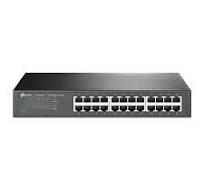
\includegraphics[width=0.58\textwidth]{switch.jpeg}

		\vfill

		\begin{latin}
			{\Large Prepared for\par}
			\vspace{0.3cm}
			{\LARGE\bfseries VAF Co.\par}
		\end{latin}

		\vspace{0.5cm}

		{\large \lr{Version 1.0}\par}
		\vspace{0.4cm}
		{\large \today\par}
	\end{titlepage}

	\pagenumbering{roman}

	\chapter*{پیشگفتار}
	\addcontentsline{toc}{chapter}{پیشگفتار}

	این راهنما برای پیکربندی، مدیریت، پایش و عیب‌یابی
	سوییچ مدیریتی \lr{DT7429 Layer 2} تهیه شده است. ساختار فصل‌ها
	با الگوی رایج راهنماهای پیکربندی \lr{Cisco Catalyst 2960} تنظیم
	شده و در آن، اصطلاحات فنی، نام قابلیت‌ها و دستورهای \lr{CLI}
	به زبان اصلی حفظ شده‌اند.

	\begin{notebox}{راهنمای استفاده}
		برای هر قابلیت، ابتدا مفهوم و پیش‌فرض‌ها، سپس دستورهای
		پیکربندی، مثال عملی و در پایان دستورهای بررسی ارائه می‌شود.
		بخش‌هایی که هنوز محتوای اختصاصی \lr{DT7429} برای آن‌ها تهیه نشده
		است، به‌صورت بخش خالی مشخص شده‌اند تا بعداً تکمیل شوند.
	\end{notebox}

	\clearpage
	\tableofcontents
	\clearpage

	\pagenumbering{arabic}

	% ============================================================================
	% فصل 1: نمای کلی و روش استفاده از CLI
	% ============================================================================
	\chapter{نمای کلی و روش استفاده از CLI}

	\section{معرفی سوییچ \lr{DT7429}}
		
		سوییچ \lr{DT7429} یک سوییچ مدیریتی لایه~2 گیگابیتی با قابلیت
		\lr{PoE} است که به‌صورت مستقل توسعه یافته و برای استفاده در شبکه‌های
		سازمانی، نظارتی، صنعتی و زیرساخت‌های ارتباطی طراحی شده است.
		
		این محصول در دو نسخه با تعداد پورت‌های متفاوت ارائه می‌شود:
		
		\begin{itemize}
			\item نسخه \lr{8-Port}: دارای 8 پورت گیگابیتی \lr{RJ45 1000Base-T}
			و 2 پورت فیبر نوری \lr{SFP 1000Base-X}.
			
			\item نسخه \lr{24-Port}: دارای 24 پورت گیگابیتی \lr{RJ45 1000Base-T}
			و 2 پورت فیبر نوری \lr{SFP 1000Base-X}.
		\end{itemize}
		
		پورت‌های اترنت این سوییچ از استانداردهای \lr{IEEE 802.3af} و
		\lr{IEEE 802.3at} برای تأمین توان از طریق شبکه، یعنی \lr{PoE}،
		پشتیبانی می‌کنند. بنابراین می‌توان تجهیزاتی مانند دوربین‌های تحت شبکه،
		تلفن‌های \lr{IP}، Access Pointها و سایر تجهیزات سازگار با \lr{PoE} را
		بدون نیاز به منبع تغذیه محلی، از طریق کابل شبکه تغذیه کرد.
		
		حداکثر توان قابل ارائه توسط هر پورت \lr{PoE} برابر با \lr{30W} است.
		حداکثر بودجه توان \lr{PoE} کل سوییچ، بسته به مدل و منبع تغذیه مورد
		استفاده، می‌تواند تا \lr{130W} یا \lr{250W} باشد.
		
		

	\section{قابلیت‌ها و ویژگی‌های سوییچ}
	
	سوییچ \lr{DT7429} یک سوییچ مدیریتی لایه~2 با قابلیت \lr{PoE} است که
	امکانات موردنیاز برای ایجاد شبکه‌ای پایدار، امن و قابل مدیریت را فراهم
	می‌کند. این سوییچ از مدیریت VLAN، جلوگیری از Loop، کنترل دسترسی،
	پایش ترافیک و ابزارهای عیب‌یابی شبکه پشتیبانی می‌کند.
	
	\begin{itemize}
		\item \textbf{مدیریت VLAN:}
		پشتیبانی از \lr{Tagged VLAN}، \lr{Untagged VLAN}، \lr{Native VLAN}،
		\lr{Private VLAN} و \lr{Virtual Interface}.
		
		\item \textbf{پایداری و جلوگیری از Loop:}
		پشتیبانی از \lr{RSTP}، \lr{MSTP}، \lr{Root Guard}،
		\lr{BPDU Guard}، \lr{Loop Guard} و \lr{UDLD}.
		
		\item \textbf{افزونگی لینک:}
		پشتیبانی از \lr{EtherChannel} و \lr{Link Aggregation} با قابلیت
		\lr{LACP}.
		
		\item \textbf{امنیت و کنترل دسترسی:}
		شامل \lr{ACL} و \lr{Extended ACL}، \lr{Port Security}،
		\lr{DHCP Snooping}، \lr{IEEE 802.1X}، \lr{AAA} و
		\lr{Privilege Modes}.
		
		\item \textbf{مدیریت ترافیک و مانیتورینگ:}
		پشتیبانی از \lr{Multicast}، \lr{IGMP Snooping}، \lr{SPAN}،
		\lr{RSPAN}، \lr{sFlow}، \lr{SNMP}، \lr{RMON} و \lr{Syslog}.
		
		\item \textbf{مدیریت شبکه:}
		پشتیبانی از \lr{DHCP Server}، \lr{DHCP Client}، \lr{NTP}،
		\lr{Ping}، \lr{Telnet} و \lr{Traceroute}.
		
		\item \textbf{پایش و عیب‌یابی:}
		پشتیبانی از \lr{SFP Monitoring} برای بررسی وضعیت ماژول‌های فیبر
		و \lr{TDR} برای تشخیص مشکلات کابل شبکه.
		
		\item \textbf{تغذیه PoE:}
		پشتیبانی از استانداردهای \lr{IEEE 802.3af/at} برای تأمین برق
		تجهیزات سازگار با \lr{PoE} از طریق پورت شبکه.
	\end{itemize}
	

	\section{پیکربندی پیش‌فرض}
	بررسی میدانی در تاریخ \lr{2026-08-22} روی دستگاه
	\lr{DT7429-8GE-2GF} با نسخه نرم‌افزار \lr{V01} انجام شد. خروجی
	\lr{show vlan} نشان داد که فقط \lr{VLAN 1} با نام \lr{default} وجود
	دارد و در شروع کار هیچ پورت access یا trunk به آن گزارش نشده است.
	در خروجی \lr{show running-config}، پورت‌های گیگابیتی در حالت
	\lr{access}، قابلیت \lr{Port Security} و \lr{UDLD} غیرفعال، و
	\lr{Dot1X} نیز غیرفعال بودند. مقدار پیش‌فرض \lr{Port-Security
	Maximum} برابر ۱ گزارش شد.

	\begin{notebox}{نکته درباره نسخه نرم‌افزار}
		فهرست دستورها به نسخه نرم‌افزار وابسته است. خروجی‌های این راهنما
		برای \lr{DT7429-8GE-2GF, V01} ثبت شده‌اند؛ در مدل یا نسخه‌ای دیگر
		ممکن است برخی شاخه‌ها یا گزینه‌ها اضافه یا حذف شده باشند.
	\end{notebox}

	\section{روند کلی پیکربندی}
	روند معمول کار به‌صورت زیر است:
	\begin{enumerate}
		\item در حالت \lr{privileged EXEC} با دستور \lr{configure terminal}
			وارد حالت پیکربندی شوید.
		\item با \lr{interface vlan <vid>} یا دستورهای پورت، اینترفیس
			موردنظر را انتخاب کنید.
		\item برای مشاهده نحو معتبر هر شاخه، در همان سطح عبارت
			\lr{<command> ?} را وارد کنید.
		\item تغییرات را با دستورهای \lr{show} بررسی و در پایان در
			حافظه راه‌اندازی ذخیره کنید.
	\end{enumerate}

	\section{حالت‌های مختلف CLI}
	سه سطح اصلی در آزمون CLI مشاهده شد:
	\begin{itemize}
		\item \lr{dt7429\#}: حالت \lr{privileged EXEC} برای دستورهای
		نمایشی مانند \lr{show} و ورود به پیکربندی.
		\item \lr{dt7429(config)\#}: حالت پیکربندی سراسری؛ شاخه‌هایی
		مانند \lr{vlan}، \lr{spanning-tree}، \lr{ntp} و \lr{snmp-server}
		در این سطح در دسترس هستند.
		\item \lr{dt7429(config-if)\#}: حالت پیکربندی اینترفیس؛
		دستورهای \lr{switchport}، \lr{ip}، \lr{qos} و \lr{spanning-tree}
		در این سطح قرار دارند.
	\end{itemize}
	دستور \lr{exit} یک سطح به عقب می‌رود و \lr{end} مستقیماً به
	\lr{privileged EXEC} بازمی‌گردد. دستور \lr{do <show-command>} برای
	اجرای دستور نمایشی از حالت پیکربندی قابل استفاده است.

	\section{نحو دستورها و روش بررسی تنظیمات}
	راهنمای درون‌خطی با علامت سؤال فعال می‌شود؛ برای نمونه:
	\begin{LTR}
		\begin{lstlisting}
			dt7429# show ?
			dt7429# show ip ?
			dt7429(config)# spanning-tree ?
			dt7429(config-if)# switchport ?
		\end{lstlisting}
	\end{LTR}
	در صورت نمایش پیام \lr{-- More --}، کلید \lr{Enter} صفحه بعد و
	کلید \lr{q} خروج از نمایش صفحه‌بندی‌شده را انجام می‌دهد. برای
	بررسی تغییرات از \lr{show running-config}، \lr{show vlan}،
	\lr{show interface status} و \lr{show ip interface brief} استفاده
		کنید.

	% ============================================================================
	% فصل 2: مدیریت IP و سرویس‌های پایه
	% ============================================================================
	\chapter{مدیریت IP و سرویس‌های پایه}

	\section{مدیریت سوییچ از طریق Interface VLAN}
	محتوای اختصاصی این بخش در فصل «تنظیمات IP و Gateway» موجود است.

	\section{تنظیم IP Address و Default Gateway}
	محتوای اختصاصی این بخش در فصل «تنظیمات IP و Gateway» موجود است.

	\section{DHCP Client}
	محتوای اختصاصی این بخش در فصل «DHCP Server و DHCP Client» موجود است.

	\section{NTP}
	محتوای اختصاصی این بخش در فصل «تنظیم و فعال‌سازی NTP» موجود است.

	\section{مدیریت از طریق SNMP و Syslog}
	برای پایش متمرکز، سوییچ شاخه‌های \lr{SNMP} و \lr{Syslog} را در
	حالت پیکربندی سراسری ارائه می‌کند. نحو دقیق برخی گزینه‌ها به نسخه
	نرم‌افزار وابسته است؛ در دستگاه آزموده‌شده (\lr{DT7429-8GE-2GF,
	V01}) پیش از تکمیل هر دستور، علامت سؤال را در همان سطح وارد کنید.

	\subsection{تنظیم SNMP}
	برای تعریف یک Community، از دستور زیر استفاده کنید:
	\begin{LTR}
		\begin{lstlisting}
			dt7429(config)# snmp-server community <name> RO
			dt7429(config)# snmp-server community <name> RW
		\end{lstlisting}
	\end{LTR}
	سطح \lr{RO} برای پایش فقط‌خواندنی و سطح \lr{RW} برای دسترسی
	خواندن/نوشتن است. Community را مانند گذرواژه در نظر بگیرید و از
	مقادیر قابل حدس استفاده نکنید. پس از اعمال تنظیمات، با
	\lr{show running-config} وجود Community را بررسی کنید و از سامانه
	مدیریت شبکه یک درخواست آزمایشی \lr{SNMP} ارسال کنید.

	برای تعیین میزبان مدیر SNMP و فعال‌کردن Trapهای مشاهده‌شده، از
	دستورهای زیر استفاده کنید:
	\begin{LTR}
		\begin{lstlisting}
			dt7429(config)# snmp-server host <ipv4>
			dt7429(config)# snmp-server enable traps vlan-membership
			dt7429(config)# snmp-server enable traps vlancreate
			dt7429(config)# snmp-server enable traps vlandelete
		\end{lstlisting}
	\end{LTR}
	این سه Trap مربوط به تغییرات عضویت و ایجاد/حذف VLAN هستند و در
	نسخه آزموده‌شده در راهنمای \lr{snmp-server ?} نمایش داده شدند.

	\begin{cautionbox}{محدودیت نسخه}
		در پیمایش CLI، شاخه‌های \lr{aaa}، \lr{radius-server}،
		\lr{tacacs-server} و \lr{crypto} نیز نمایش داده شدند، اما
		احراز هویت SNMP، ‏\lr{SNMPv3} و جزئیات ACL در این آزمون تأیید
		نشدند. فعال‌سازی آن‌ها را فقط پس از مشاهده نحو کامل با
		\lr{snmp-server ?} و آزمون قابل بازگشت انجام دهید.
	\end{cautionbox}

	\subsection{تنظیم Syslog}
	برای ارسال پیام‌های سیستمی به یک سرور مرکزی، ابتدا سطح شدت پیام و
	سپس میزبان Syslog را تنظیم کنید:
	\begin{LTR}
		\begin{lstlisting}
			dt7429(config)# logging trap <level>
			dt7429(config)# logging host <server-ip>
		\end{lstlisting}
	\end{LTR}
	مقدار \lr{<level>} را با اجرای \lr{logging trap ?} از فهرست مجاز
	انتخاب کنید؛ سطح‌های شدیدتر پیام‌های کمتری تولید می‌کنند و سطح‌های
	پایین‌تر برای عیب‌یابی جزئیات بیشتری می‌فرستند. آدرس
	\lr{<server-ip>} باید از طریق Interface مدیریتی سوییچ قابل دسترسی
	باشد؛ در صورت قرارداشتن سرور خارج از Subnet محلی، Default Gateway
	را نیز تنظیم کنید.

	\begin{cmdtable}{SNMP and Syslog Verification}
		\texttt{show running-config} &
		Verify the configured SNMP community and Syslog destination \\

		\texttt{show logging} &
		Display local logging state and recent messages, if supported \\

		\texttt{show snmp} &
		Display SNMP state and counters, if supported \\
	\end{cmdtable}

	اگر \lr{show logging} یا \lr{show snmp} در نسخه نصب‌شده پذیرفته نشد،
	از \lr{show ?} برای یافتن شاخه معادل استفاده کنید. در پایان، خروجی
	\lr{show running-config} را ثبت و پیکربندی را در حافظه راه‌اندازی
	ذخیره کنید.

	% ============================================================================
	% فصل 3: VLAN و پورت‌های Access و Trunk
	% ============================================================================
	\chapter{پیکربندی VLAN}
	\label{chap:vlan}

	این فصل نحوه پیکربندی
	\lr{Virtual Local Area Networks (VLANs)}
	را بر روی سوییچ مدیریتی \lr{DT7429 Layer 2+} تشریح می‌کند.
	مباحث این فصل شامل \lr{port modes}، \lr{standard VLANs}،
	\lr{native VLANs} در \lr{trunk links}، \lr{voice VLANs} و
	\lr{private VLANs} است.

	استفاده از \lr{VLANs} امکان تقسیم‌بندی منطقی یک
	\lr{physical switch} به چندین \lr{broadcast domain} مستقل را فراهم
	می‌کند. این تقسیم‌بندی موجب بهبود \lr{network security}،
	ایزوله‌سازی ترافیک (\lr{traffic isolation}) و سهولت در مدیریت
	(\lr{manageability}) شبکه می‌شود.

	سوییچ \lr{DT7429} از حداکثر
	\lr{4094 IEEE 802.1Q VLANs} پشتیبانی می‌کند. همچنین قابلیت‌های
	\lr{protocol-based VLANs}، \lr{MAC-based VLANs}، \lr{voice VLANs}
	و \lr{QinQ (802.1Q tunneling)} در این دستگاه پشتیبانی می‌شوند.

	% ============================================================================
	\section{پیکربندی \lr{Switch Port Modes} (\lr{Access and Trunk})}
	\label{sec:port-modes}

	پیش از آن‌که یک \lr{VLAN} بتواند ترافیک را از طریق یک پورت منتقل کند،
	باید حالت عملکرد پورت به یکی از دو حالت \lr{access} یا \lr{trunk}
	تنظیم شود. پورت‌های \lr{Access} تنها ترافیک یک \lr{VLAN} را حمل
	می‌کنند و معمولاً برای اتصال تجهیزات انتهایی نظیر رایانه، چاپگر و
	\lr{IP phone} استفاده می‌شوند. پورت‌های \lr{Trunk} ترافیک برچسب‌گذاری‌شده
	(\lr{tagged traffic}) مربوط به چندین \lr{VLAN} را حمل می‌کنند و
	عموماً برای اتصال بین سوییچ‌ها یا اتصال سوییچ به روتر کاربرد دارند.

	حالت پورت در \lr{interface configuration mode} و با استفاده از
	خانواده دستورهای \lr{\texttt{switchport}} پیکربندی می‌شود. افزودن
	\lr{\texttt{no}} در ابتدای هر یک از این دستورها، تنظیم مربوطه را به
	مقدار پیش‌فرض بازمی‌گرداند.

	\begin{cautionbox}{\lr{Caution}}
		برخلاف برخی پلتفرم‌های سوییچ، دستگاه \lr{DT7429} در زمان فعال‌سازی
		حالت \lr{trunk}، حالت پیش‌فرض \lr{``allow all''} را پیاده‌سازی
		نمی‌کند. باید \lr{VLAN}های مجاز به‌صورت صریح به فهرست مجاز
		\lr{trunk} اضافه شوند؛ در غیر این صورت، هیچ ترافیک برچسب‌گذاری‌شده‌ای
		از طریق آن \lr{trunk} ارسال نخواهد شد.
	\end{cautionbox}

	\begin{cmdtable}{Access and Trunk Port Configuration Commands}
		\texttt{DT7429(config)\# interface gigabitethernet 1} &
		Enter interface configuration mode \\

		\texttt{DT7429(config-if)\# switchport mode access} &
		Set the port to access mode \\

		\texttt{DT7429(config-if)\# no switchport mode access} &
		Remove access mode from the port \\

		\texttt{DT7429(config-if)\# switchport access vlan \textit{vlan-id}} &
		Assign an access port to a VLAN \\

		\texttt{DT7429(config-if)\# switchport mode trunk} &
		Set the port to trunk mode \\

		\texttt{DT7429(config-if)\# no switchport mode trunk} &
		Remove trunk mode from the port \\

		\texttt{DT7429(config-if)\# switchport trunk allowed vlan \textit{vlan-list}} &
		Specify VLANs allowed on the trunk\newline
		\textit{(required before tagged traffic is forwarded)} \\
	\end{cmdtable}

	\begin{notebox}{\lr{Verify Configuration}}
		برای اطمینان از اعمال شدن تغییرات مربوط به حالت پورت و
		\lr{VLAN}ها، دستور \lr{privileged EXEC} زیر را اجرا کنید:

		\begin{LTR}
			\begin{lstlisting}
				DT7429# show interface (interface-id) switchport
			\end{lstlisting}
		\end{LTR}
	\end{notebox}

	\subsection{مثال پیکربندی}

	مثال زیر، اینترفیس \lr{\texttt{GigabitEthernet2}} را به‌عنوان یک
	پورت \lr{trunk} پیکربندی کرده و عبور \lr{VLAN}های ۱، ۲، ۵ و ۶ را
	مجاز می‌کند:

	\begin{LTR}
		\begin{lstlisting}
			DT7429(config)# interface gigabitethernet2
			DT7429(config-if)# switchport mode trunk
			DT7429(config-if)# switchport trunk allowed vlan add 1,2,5,6
		\end{lstlisting}
	\end{LTR}

	% ============================================================================
	\section{\lr{Configuring VLANs}}
	\label{sec:vlan-basic}

	ایجاد \lr{VLAN}ها در \lr{global configuration mode} انجام می‌شود.
	هر \lr{VLAN} با یک شناسه عددی \lr{VLAN ID} مشخص شده و می‌تواند
	به‌صورت اختیاری دارای یک نام توصیفی باشد. قرار دادن
	\lr{\texttt{no}} قبل از دستور \lr{\texttt{vlan}}، \lr{VLAN} مشخص‌شده
	را حذف می‌کند.

	\begin{cmdtable}{Basic VLAN Configuration Commands}
		\texttt{DT7429(config)\# vlan \textit{vlan-id}} &
		Create a VLAN and enter VLAN configuration mode \\

		\texttt{DT7429(config)\# no vlan \textit{vlan-id}} &
		Delete a VLAN \\

		\texttt{DT7429(config-vlan)\# name \textit{Engineering}} &
		Assign a name to the VLAN (1--32 characters) \\

		\texttt{DT7429(config-vlan)\# exit} &
		Apply changes and return to global configuration mode \\
	\end{cmdtable}

	\begin{cmdtable}{Displaying VLAN Information}
		\texttt{DT7429\# show vlan} &
		Display all configured VLANs \\
	\end{cmdtable}

	\begin{notebox}{\lr{Default Behavior}}
		\begin{itemize}[leftmargin=1.4em, itemsep=2pt]
			\item به‌صورت پیش‌فرض، همه پورت‌های سوییچ عضو \lr{\textbf{VLAN 1}} هستند.
			\item \lr{\textbf{VLAN 1}}، \lr{VLAN} پیش‌فرض است و قابل حذف نیست.
		\end{itemize}
	\end{notebox}

	% ============================================================================
	\section{\lr{Configuring the Native VLAN}}
	\label{sec:native-vlan}

	در یک لینک \lr{IEEE 802.1Q trunk}، ترافیک بدون برچسب
	(\lr{untagged traffic}) از طریق \lr{native VLAN} منتقل می‌شود.
	به‌صورت پیش‌فرض، \lr{VLAN 1} به‌عنوان \lr{native VLAN} در کل سوییچ
	استفاده می‌شود. در این بخش نحوه تغییر \lr{native VLAN} روی یک
	اینترفیس \lr{trunk} توضیح داده می‌شود.

	\begin{notebox}{\lr{Default Behavior}}
		\begin{itemize}[leftmargin=1.4em, itemsep=2pt]
			\item به‌صورت پیش‌فرض، تمام اینترفیس‌های سوییچ عضو \lr{\textbf{VLAN 1}} هستند.
			\item به‌صورت پیش‌فرض، \lr{native VLAN} کل سوییچ برابر با \lr{\textbf{VLAN 1}} است.
			\item تغییرات \lr{native VLAN} تنها پس از اعمال پیکربندی
			\lr{\texttt{interface GigabitEthernet}} مربوطه فعال می‌شوند.
		\end{itemize}
	\end{notebox}

	\subsection{\lr{Native VLAN Configuration Procedure}}

	\begin{enumerate}[leftmargin=1.6em]

		\item \textbf{ایجاد \lr{native VLAN} جدید.}
		برای مثال، جهت ایجاد \lr{VLAN 10}:

		\begin{LTR}
			\begin{lstlisting}
				DT7429# configure terminal
				DT7429(config)# vlan 10
			\end{lstlisting}
		\end{LTR}

		\item \textbf{ورود به اینترفیس \lr{trunk} موردنظر.}
		تنظیم \lr{native VLAN} فقط روی اینترفیس‌های \lr{trunk} اعمال می‌شود.
		بنابراین ابتدا باید پورت در حالت \lr{trunk} پیکربندی شود:

		\begin{LTR}
			\begin{lstlisting}
				DT7429# configure terminal
				DT7429(config)# interface gigabitethernet 10
				DT7429(config-if)# switchport mode trunk
			\end{lstlisting}
		\end{LTR}

		\item \textbf{تغییر \lr{native VLAN}.}
		دستور زیر \lr{native VLAN} را از مقدار پیش‌فرض \lr{VLAN 1} به
		\lr{VLAN 10} تغییر می‌دهد:

		\begin{LTR}
			\begin{lstlisting}
				DT7429(config-if)# switchport trunk native vlan 10
				DT7429(config-if)# exit
			\end{lstlisting}
		\end{LTR}

	\end{enumerate}

	% ============================================================================
	\section{پیکربندی Voice VLAN}
	\label{sec:voice-vlan}

	قابلیت \lr{Voice VLAN} امکان جداسازی خودکار ترافیک تلفن‌های
	\lr{IP} از ترافیک داده را روی یک پورت \lr{access} مشترک فراهم
	می‌کند. این قابلیت، اعمال سیاست‌های \lr{QoS} را ساده‌تر کرده و
	کیفیت ترافیک صوتی را بهبود می‌دهد. \lr{Voice VLAN} در
	\lr{interface configuration mode} و با دستور
	\lr{\texttt{switchport voice vlan}} فعال می‌شود. افزودن
	\lr{\texttt{no}} در ابتدای دستور، آن را غیرفعال می‌کند.

	\begin{cmdtable}{Voice VLAN Configuration Commands}
		\texttt{DT7429(config)\# interface \textit{interface-id}} &
		Enter the target interface \\

		\texttt{DT7429(config-if)\# switchport voice vlan \textit{vlan-id}} &
		Assign the VLAN used to carry voice traffic \\

		\texttt{DT7429(config-if)\# no switchport voice vlan \textit{vlan-id}} &
		Remove the voice VLAN assignment \\

		\texttt{DT7429(config-if)\# switchport voice vlan untagged} &
		Configure IP phones to send untagged frames\newline
		\textit{(default mode for all phones)} \\
	\end{cmdtable}

	\begin{cautionbox}{\lr{Requirement}}
		قابلیت \lr{Voice VLAN} باید روی یک پورت \lr{Layer 2} که در حالت
		\lr{\textbf{access}} فعالیت می‌کند پیکربندی شود.
	\end{cautionbox}

	\subsection{مثال پیکربندی}

	مثال زیر \lr{VLAN 2} را به‌عنوان \lr{voice VLAN} روی اینترفیس
	\lr{\texttt{GigabitEthernet2}} اختصاص می‌دهد:

	\begin{LTR}
		\begin{lstlisting}
			DT7429(config)# interface gigabitethernet2
			DT7429(config-if)# switchport voice vlan 2
		\end{lstlisting}
	\end{LTR}

	% ============================================================================
	\section{\lr{Configuring Private VLANs}}
	\label{sec:private-vlan}

	قابلیت \lr{Private VLANs (PVLANs)} امکان ایزوله‌سازی در لایه ۲ را
	بین پورت‌هایی که در یک \lr{primary VLAN} مشترک قرار دارند، فراهم
	می‌کند. یک \lr{private VLAN} شامل یک \lr{primary VLAN} و یک یا چند
	\lr{secondary VLAN} است. هر \lr{secondary VLAN} می‌تواند در یکی از
	حالت‌های زیر فعالیت کند:

	\begin{itemize}[leftmargin=1.4em]
		\item \textbf{\lr{Isolated}} ---
		میزبان‌ها فقط می‌توانند با پورت‌های \lr{promiscuous} ارتباط برقرار کنند.
		میزبان‌های \lr{isolated} نمی‌توانند با یکدیگر ارتباط داشته باشند.

		\item \textbf{\lr{Community}} ---
		میزبان‌ها می‌توانند با سایر اعضای همان \lr{community} و همچنین پورت‌های
		\lr{promiscuous} ارتباط برقرار کنند.

		\item \textbf{\lr{Promiscuous}} ---
		معمولاً پورت \lr{uplink} یا پورت متصل به روتر است و می‌تواند با تمام
		میزبان‌های \lr{isolated} و \lr{community} ارتباط برقرار کند.
	\end{itemize}

	\begin{cmdtable}{Private VLAN Port Configuration Commands}
		\texttt{DT7429(config-if)\# switchport mode private-vlan \{host \textbar\ promiscuous\}} &
		Set the private VLAN port mode \\

		\texttt{DT7429(config-if)\# switchport private-vlan host-association \textit{vid}} &
		Associate a host port with a secondary VLAN \\

		\texttt{DT7429(config-if)\# switchport private-vlan mapping \{add \textbar\ remove\} \textit{secondary-vlan-list}} &
		Map or unmap secondary VLANs to the primary VLAN\newline
		\textit{(configured on the promiscuous/uplink port)} \\
	\end{cmdtable}

	\subsection{مثال پیکربندی}

	مثال زیر یک \lr{isolated secondary VLAN} با شناسه \lr{200} و پورت‌های
	عضو \lr{\texttt{GigabitEthernet1--2}} ایجاد می‌کند. همچنین یک
	\lr{community secondary VLAN} با شناسه \lr{300} و پورت‌های عضو
	\lr{\texttt{GigabitEthernet3--4}} پیکربندی می‌شود:

	\begin{LTR}
		\begin{lstlisting}
			DT7429# configure terminal
			DT7429(config)# vlan 200
			DT7429(config-vlan)# private-vlan isolated
			DT7429(config-vlan)# exit
			DT7429(config)# interface range GigabitEthernet 1-2
			DT7429(config-if-range)# switchport mode access
			DT7429(config-if-range)# switchport private-vlan host-association 200
			DT7429(config-if-range)# exit
			DT7429(config)# vlan 300
			DT7429(config-vlan)# private-vlan community
			DT7429(config-vlan)# exit
			DT7429(config)# interface range GigabitEthernet 3-4
			DT7429(config-if-range)# switchport private-vlan host-association 300
			DT7429(config-if-range)# end
		\end{lstlisting}
	\end{LTR}

	\subsection{\lr{Verification}}

	برای بررسی پیکربندی \lr{Private VLAN}، دستور زیر را اجرا کنید:

	\begin{LTR}
		\begin{lstlisting}
			DT7429# show vlan private-vlan

			VLAN   PVLAN_NO   community_ports
			----   --------   ---------------
			300    1          3,4

			VID    isolated_ports
			----   --------------
			200    1,2
		\end{lstlisting}
	\end{LTR}

	\section{پیکربندی گروهی با \lr{Interface Range}}

	برای اعمال یک تنظیم یکسان روی چند پورت، از حالت
	\lr{config-if-range} استفاده کنید:

	\begin{LTR}
		\begin{lstlisting}
			DT7429(config)# interface range GigabitEthernet 1-9
			DT7429(config-if-range)# switchport mode access
			DT7429(config-if-range)# switchport access vlan 10
		\end{lstlisting}
	\end{LTR}

	برای انتخاب پورت‌های غیرپیوسته، شناسه‌ها را با ویرگول جدا کنید:

	\begin{LTR}
		\begin{lstlisting}
			DT7429(config)# interface range GigabitEthernet 1,3,5
		\end{lstlisting}
	\end{LTR}

	پیش از اعمال تنظیم، وجود همه پورت‌ها و سازگاری حالت فعلی آن‌ها را
	بررسی کنید. برای بازگشت به حالت پیکربندی سراسری، \lr{exit} یا
	\lr{end} را اجرا کنید. این دستورها در نسخه آزموده‌شده در
	\lr{interface ?} با الگوهای \lr{n|1-26|1,2,..} اعلام شدند.

	\chapter{پیکربندی Spanning Tree Protocol (STP)}

	پروتکل \lr{Spanning Tree Protocol (STP)} برای جلوگیری از ایجاد
	\lr{Layer 2 Loop} در شبکه استفاده می‌شود. در شبکه‌هایی که بین
	سوییچ‌ها مسیرهای افزونه وجود دارد، ممکن است فریم‌های \lr{Broadcast}
	یا \lr{Unknown Unicast} به‌صورت نامحدود در شبکه گردش کنند.

	STP با بررسی توپولوژی شبکه، مسیرهای اضافی را به‌صورت منطقی
	غیرفعال می‌کند و تنها یک مسیر مناسب را در حالت \lr{Forwarding}
	نگه می‌دارد. در صورت قطع مسیر اصلی، یکی از مسیرهای جایگزین
	می‌تواند دوباره فعال شود.

	\begin{tipbox}{نکته مدیریتی}
		پیش از فعال‌سازی STP، توپولوژی فیزیکی شبکه، مسیرهای افزونه و
		نقش هر سوییچ در شبکه را بررسی کنید. تغییر نادرست در
		\lr{STP Mode} یا \lr{Bridge Priority} ممکن است باعث تغییر
		مسیر عبور ترافیک شود.
	\end{tipbox}


	% ============================================================================
	\section{فعال‌سازی و تنظیمات Global مربوط به STP}
	% ============================================================================

	فعال‌سازی STP در سطح Global باعث می‌شود پروتکل روی سوییچ فعال شود
	و سوییچ بتواند در فرایند انتخاب \lr{Root Bridge} و محاسبه مسیرهای
	مناسب شرکت کند.

	در حالت عادی، STP باید روی تمام سوییچ‌هایی که در یک توپولوژی
	افزونه قرار دارند فعال باشد. غیرفعال‌کردن STP فقط در شرایط خاص
	و پس از اطمینان از نبود مسیر حلقه‌ای مجاز است.

	\begin{latin}
		\begin{lstlisting}[language=bash]
			DT7429(config)# spanning-tree enable
			DT7429(config)# no spanning-tree enable
		\end{lstlisting}
	\end{latin}

	\begin{cmdtable}{Global Spanning Tree Configuration Commands}
		\texttt{DT7429(config)\# spanning-tree enable} &
		Enable Spanning Tree Protocol globally \\

		\texttt{DT7429(config)\# no spanning-tree enable} &
		Disable Spanning Tree Protocol globally \\

		\texttt{DT7429(config)\# spanning-tree mode
			\textit{\{stp | rstp | mstp\}}} &
		Select the global Spanning Tree operating mode \\

		\texttt{DT7429\# show spanning-tree} &
		Display global Spanning Tree status and interface details \\
	\end{cmdtable}

	\begin{cautionbox}{هشدار}
		غیرفعال‌کردن STP روی سوییچی که دارای لینک‌های افزونه است،
		می‌تواند باعث ایجاد \lr{Layer 2 Loop} و اختلال گسترده در شبکه شود.
		قبل از استفاده از دستور \lr{no spanning-tree enable}، از نبود
		مسیر حلقه‌ای اطمینان حاصل کنید.
	\end{cautionbox}


	% ============================================================================
	\section{انتخاب STP Mode}
	% ============================================================================

	سوییچ DT7429 می‌تواند در یکی از حالت‌های استاندارد
	\lr{STP}، \lr{RSTP} یا \lr{MSTP} فعالیت کند. انتخاب حالت مناسب
	به اندازه و پیچیدگی شبکه، تعداد \lr{VLAN}ها و نیازمندی‌های
	همگرایی شبکه بستگی دارد.

	\begin{table}[htbp]
		\centering
		\caption{Spanning Tree Operating Modes}
		\label{tab:stp-operating-modes}
		\begin{tabular}{|p{3.2cm}|p{4.5cm}|p{5.0cm}|}
			\hline
			\textbf{Mode} &
			\textbf{Description} &
			\textbf{Recommended Use} \\
			\hline
			\texttt{STP} &
			Legacy Spanning Tree mode with standard convergence behavior &
			Legacy or compatibility environments \\
			\hline
			\texttt{RSTP} &
			Rapid Spanning Tree mode with faster convergence &
			Small and medium networks requiring rapid recovery \\
			\hline
			\texttt{MSTP} &
			Maps multiple VLANs to Spanning Tree instances &
			Large networks with multiple VLANs and redundant links \\
			\hline
		\end{tabular}
	\end{table}

	برای تغییر حالت کاری STP، از دستورات زیر استفاده کنید:

	\begin{latin}
		\begin{lstlisting}[language=bash]
			DT7429(config)# spanning-tree mode stp
			DT7429(config)# spanning-tree mode rstp
			DT7429(config)# spanning-tree mode mstp
		\end{lstlisting}
	\end{latin}

	\begin{tipbox}{پیشنهاد پیکربندی}
		در شبکه‌هایی که به همگرایی سریع نیاز دارند، استفاده از
		\lr{RSTP} یا \lr{MSTP} نسبت به \lr{STP} معمولی پیشنهاد می‌شود.
		در صورت استفاده از \lr{MSTP}، تنظیمات \lr{MST Region} باید روی
		تمام سوییچ‌های عضو یک Region یکسان باشد.
	\end{tipbox}


	% ============================================================================
	\section{پیکربندی Interface و Edge Port}
	% ============================================================================

	پورت‌هایی که به تجهیزات نهایی مانند کامپیوتر، تلفن تحت شبکه،
	دوربین یا سرور متصل هستند، معمولاً نباید مانند لینک بین دو
	سوییچ در فرایند STP رفتار کنند. این پورت‌ها به‌عنوان
	\lr{Edge Port} شناخته می‌شوند.

	قرار‌دادن یک پورت در حالت \lr{Edge} باعث می‌شود پورت سریع‌تر
	وارد حالت \lr{Forwarding} شود. این قابلیت برای کاهش زمان انتظار
	تجهیزات نهایی هنگام برقراری اتصال استفاده می‌شود.

	\begin{cmdtable}{Interface Spanning Tree Configuration Commands}
		\texttt{DT7429(config)\# interface
			\textit{GigabitEthernet/interface-id}} &
		Enter interface configuration mode \\

		\texttt{DT7429(config-if)\# spanning-tree ?} &
		Display available Spanning Tree interface commands \\

		\texttt{DT7429(config-if)\# spanning-tree edge} &
		Enable administrative edge mode on the interface \\

		\texttt{DT7429(config-if)\# spanning-tree auto-edge} &
		Enable automatic edge-port detection \\

		\texttt{DT7429(config-if)\# spanning-tree port-priority
			\textit{priority}} &
		Change the Spanning Tree port priority \\

		\texttt{DT7429(config-if)\# do show spanning-tree} &
		Display Spanning Tree information without leaving interface mode \\
	\end{cmdtable}

	\begin{table}[htbp]
		\centering
		\caption{Edge Port Operating Modes}
		\label{tab:edge-port-modes}
		\begin{tabular}{|p{3.0cm}|p{5.0cm}|p{4.7cm}|}
			\hline
			\textbf{Mode} &
			\textbf{Behavior} &
			\textbf{Typical Application} \\
			\hline
			\texttt{Default} &
			The port participates in the standard Spanning Tree process &
			Switch-to-switch links and network infrastructure \\
			\hline
			\texttt{Auto-edge} &
			The switch detects whether the port is connected to an edge
			device or another Spanning Tree device &
			Ports with an unknown or changing connection type \\
			\hline
			\texttt{Edge} &
			The port immediately transitions to the forwarding state,
			unless a BPDU is received &
			Ports connected to PCs, servers, IP phones, or cameras \\
			\hline
		\end{tabular}
	\end{table}

	نمونهٔ زیر، یک پورت را به‌عنوان \lr{Edge Port} تنظیم می‌کند:

	\begin{latin}
		\begin{lstlisting}[language=bash]
			DT7429(config)# interface GigabitEthernet 2
			DT7429(config-if)# spanning-tree edge
		\end{lstlisting}
	\end{latin}

	در صورتی که نوع تجهیز متصل به پورت مشخص نباشد، می‌توان از
	\lr{Auto-edge} استفاده کرد. این حالت با بررسی دریافت یا عدم دریافت
	\lr{BPDU}، دربارهٔ Edge یا Non-edge بودن پورت تصمیم‌گیری می‌کند.

	\begin{latin}
		\begin{lstlisting}[language=bash]
			DT7429(config)# interface GigabitEthernet 2
			DT7429(config-if)# spanning-tree auto-edge
		\end{lstlisting}
	\end{latin}

	\begin{cautionbox}{هشدار}
		حالت \lr{Edge} را روی لینک‌های بین سوییچ‌ها، لینک‌های
		\lr{Trunk} یا پورت‌هایی که احتمال اتصال سوییچ به آن‌ها وجود دارد
		فعال نکنید؛ زیرا این کار می‌تواند پورت را بدون تأخیر وارد حالت
		\lr{Forwarding} کند و احتمال ایجاد Loop را افزایش دهد.
	\end{cautionbox}


	% ============================================================================
	\section{BPDU Guard و BPDU Filter}
	% ============================================================================

	پیام‌های \lr{Bridge Protocol Data Unit (BPDU)} برای تبادل اطلاعات
	بین سوییچ‌ها و محاسبه توپولوژی STP استفاده می‌شوند. روی پورت‌هایی
	که به تجهیزات نهایی متصل هستند، دریافت BPDU می‌تواند نشانهٔ اتصال
	یک سوییچ یا تجهیز غیرمجاز باشد.

	قابلیت‌های \lr{BPDU Guard} و \lr{BPDU Filter} برای محافظت از
	پورت‌های Edge استفاده می‌شوند، اما عملکرد آن‌ها یکسان نیست.

	\begin{table}[htbp]
		\centering
		\caption{BPDU Protection Features}
		\label{tab:bpdu-protection}
		\begin{tabular}{|p{3.0cm}|p{5.0cm}|p{4.7cm}|}
			\hline
			\textbf{Feature} &
			\textbf{Behavior} &
			\textbf{Recommended Use} \\
			\hline
			\texttt{BPDU Guard} &
			Disables or error-disables the port when a BPDU is received &
			Access ports connected to trusted end devices \\
			\hline
			\texttt{BPDU Filter} &
			Filters BPDU transmission or reception on the interface &
			Special-purpose edge ports requiring BPDU suppression \\
			\hline
		\end{tabular}
	\end{table}

	برای تنظیم این قابلیت‌ها، ابتدا وارد پیکربندی پورت شوید:

	\begin{latin}
		\begin{lstlisting}[language=bash]
			DT7429(config)# interface GigabitEthernet 2
			DT7429(config-if)# spanning-tree edge
			DT7429(config-if)# spanning-tree bpdu-guard enable
			DT7429(config-if)# spanning-tree bpdu-filter enable
		\end{lstlisting}
	\end{latin}

	\begin{cautionbox}{تفاوت BPDU Guard و BPDU Filter}
		در صورت دریافت BPDU، قابلیت \lr{BPDU Guard} برای حفاظت از شبکه
		پورت را غیرفعال می‌کند؛ اما \lr{BPDU Filter} پیام‌های BPDU را
		فیلتر می‌کند و ممکن است از مشارکت پورت در فرایند تشخیص توپولوژی
		جلوگیری کند. استفاده از \lr{BPDU Filter} باید با دقت انجام شود.
	\end{cautionbox}


	% ============================================================================
	\section{Loop Guard}
	% ============================================================================

	قابلیت \lr{Loop Guard} برای شناسایی شرایطی مانند
	\lr{Unidirectional Link} استفاده می‌شود. در این شرایط ممکن است
	پورت، پیام‌های BPDU را دریافت نکند و به‌اشتباه وارد حالت
	\lr{Forwarding} شود.

	\lr{Loop Guard} با قرار‌دادن پورت مشکوک در حالت
	\lr{Loop-inconsistent} از ایجاد Loop جلوگیری می‌کند. این قابلیت
	به‌ویژه برای لینک‌های بین سوییچ‌ها و مسیرهای افزونه اهمیت دارد.

	\begin{cmdtable}{Loop Guard Configuration Commands}
		\texttt{DT7429(config-if)\# spanning-tree auto-edge} &
		Enable automatic edge-port detection before applying Loop Guard \\

		\texttt{DT7429(config-if)\# spanning-tree guard loop} &
		Enable Loop Guard on the selected interface \\

		\texttt{DT7429(config-if)\# do show spanning-tree} &
		Display the current interface Spanning Tree state \\
	\end{cmdtable}

	نمونهٔ پیکربندی \lr{Loop Guard} به‌صورت زیر است:

	\begin{latin}
		\begin{lstlisting}[language=bash]
			DT7429(config)# interface GigabitEthernet 2
			DT7429(config-if)# spanning-tree auto-edge
			DT7429(config-if)# spanning-tree guard loop
		\end{lstlisting}
	\end{latin}

	\begin{tipbox}{نکته عملیاتی}
		پس از فعال‌سازی \lr{Loop Guard}، وضعیت پورت را با دستور
		\lr{show spanning-tree} بررسی کنید. در صورت تشخیص مشکل در لینک،
		ممکن است پورت در حالت \lr{Loop-inconsistent} قرار گیرد تا از
		عبور ترافیک و ایجاد Loop جلوگیری شود.
	\end{tipbox}


	% ============================================================================
	\section{UDLD و تشخیص لینک یک‌طرفه}
	% ============================================================================

	قابلیت \lr{Unidirectional Link Detection (UDLD)} برای تشخیص
	لینک‌هایی استفاده می‌شود که ارتباط آن‌ها فقط در یک جهت برقرار است.
	این وضعیت می‌تواند در اثر خرابی فیبر، مشکل در Transceiver یا
	اختلال در یکی از مسیرهای ارسال و دریافت ایجاد شود.

	استفاده از \lr{UDLD} در کنار \lr{STP} و \lr{Loop Guard} می‌تواند
	پایداری شبکه را در لینک‌های افزونه افزایش دهد.

	\begin{cmdtable}{UDLD Configuration Commands}
		\texttt{DT7429(config-if)\# udld port} &
		Enable UDLD on the interface \\

		\texttt{DT7429(config-if)\# exit} &
		Exit interface configuration mode \\

		\texttt{DT7429(config)\# do show interface status} &
		Display interface status and possible error-disabled state \\
	\end{cmdtable}

	نمونهٔ فعال‌سازی \lr{UDLD} روی یک پورت:

	\begin{latin}
		\begin{lstlisting}[language=bash]
			DT7429(config)# interface GigabitEthernet 2
			DT7429(config-if)# udld port
			DT7429(config-if)# exit
			DT7429(config)# do show interface status
		\end{lstlisting}
	\end{latin}


	% ============================================================================
	\section{پیکربندی MSTP}
	% ============================================================================

	پروتکل \lr{Multiple Spanning Tree Protocol (MSTP)} امکان نگاشت چند
	\lr{VLAN} به یک \lr{MST Instance} را فراهم می‌کند. در نتیجه،
	به‌جای ایجاد یک نمونهٔ مستقل از STP برای هر VLAN، چند VLAN می‌توانند
	از یک Instance مشترک استفاده کنند.

	این روش تعداد محاسبات STP را کاهش داده و امکان استفادهٔ بهتر از
	لینک‌های افزونه را فراهم می‌کند. تمام سوییچ‌هایی که در یک
	\lr{MST Region} قرار دارند باید دارای تنظیمات یکسانی برای
	\lr{Region Name}، \lr{Revision Number} و نگاشت VLANها باشند.

	\begin{cmdtable}{MSTP Configuration Commands}
		\texttt{DT7429(config)\# spanning-tree mode mstp} &
		Enable MSTP mode globally \\

		\texttt{DT7429(config)\# spanning-tree mst configuration} &
		Enter MST region configuration mode \\

		\texttt{DT7429(config-mst)\# name \textit{region-name}} &
		Assign a name to the MST region \\

		\texttt{DT7429(config-mst)\# revision
			\textit{revision-number}} &
		Assign the MST region revision number \\

		\texttt{DT7429(config-mst)\# instance
			\textit{instance-id} vlan \textit{vlan-list}} &
		Map VLANs to an MST instance \\

		\texttt{DT7429(config-mst)\# priority instance
			\textit{instance-id} set \textit{priority}} &
		Set the priority for a specific MST instance \\

		\texttt{DT7429(config-mst)\# exit} &
		Exit MST configuration mode \\

		\texttt{DT7429(config)\# do show spanning-tree} &
		Display MSTP status and instance information \\
	\end{cmdtable}

	نمونهٔ زیر دو گروه از \lr{VLAN}ها را به دو
	\lr{MST Instance} مختلف نگاشت می‌کند:

	\begin{latin}
		\begin{lstlisting}[language=bash]
			DT7429(config)# spanning-tree enable
			DT7429(config)# spanning-tree mode mstp
			DT7429(config)# spanning-tree mst configuration
			DT7429(config-mst)# name REGION1
			DT7429(config-mst)# revision 1
			DT7429(config-mst)# instance 1 vlan 10,20,30
			DT7429(config-mst)# instance 2 vlan 40,50,60
			DT7429(config-mst)# exit
			DT7429(config)# spanning-tree mst configuration
			DT7429(config-mst)# priority instance 1 set 8192
			DT7429(config-mst)# exit
		\end{lstlisting}
	\end{latin}

	\begin{tipbox}{نکته هماهنگی MST Region}
		برای عملکرد صحیح MSTP، مقادیر \lr{Region Name}،
		\lr{Revision Number} و \lr{VLAN-to-Instance Mapping} باید در
		تمام سوییچ‌های یک Region یکسان باشند. در غیر این صورت، سوییچ‌ها
		ممکن است در Regionهای متفاوت قرار بگیرند.
	\end{tipbox}


	% ============================================================================
	\section{بررسی و تأیید تنظیمات}
	% ============================================================================

	پس از اعمال تنظیمات، وضعیت STP باید بررسی شود. این بررسی شامل
	اطمینان از فعال‌بودن STP، شناسایی صحیح \lr{Root Bridge}، وضعیت
	پورت‌ها، نقش پورت‌ها و وضعیت \lr{MST Instance}ها است.

	\begin{cmdtable}{Spanning Tree Verification Commands}
		\texttt{DT7429\# show spanning-tree} &
		Display global STP or MSTP status \\

		\texttt{DT7429(config-if)\# do show spanning-tree} &
		Display Spanning Tree information from interface mode \\

		\texttt{DT7429(config)\# do show interface status} &
		Display interface operational and error-disabled states \\
	\end{cmdtable}

	نمونهٔ دستور بررسی وضعیت کلی STP:

	\begin{latin}
		\begin{lstlisting}[language=bash]
			DT7429# show spanning-tree
		\end{lstlisting}
	\end{latin}

	هنگام بررسی خروجی، موارد زیر را کنترل کنید:

	\begin{itemize}
		\item فعال‌بودن صحیح \lr{STP} یا \lr{MSTP}؛
		\item مشخص‌بودن \lr{Root Bridge}؛
		\item صحیح‌بودن نقش و وضعیت هر پورت؛
		\item قرارنداشتن پورت‌های غیرمنتظره در حالت \lr{Forwarding}؛
		\item شناسایی پورت‌های دارای وضعیت \lr{Loop-inconsistent} یا
		\lr{Error-disabled}؛
		\item یکسان‌بودن تنظیمات \lr{MST Region} در سوییچ‌های مرتبط.
	\end{itemize}

	\begin{cautionbox}{هشدار نهایی}
		پس از هر تغییر در تنظیمات STP، وضعیت لینک‌های بین سوییچ‌ها و
		مسیر عبور ترافیک را بررسی کنید. تغییر در \lr{STP Mode}،
		\lr{Port Priority} یا \lr{MST Instance Mapping} می‌تواند باعث
		انتخاب مجدد مسیرها و تغییر توپولوژی منطقی شبکه شود.
	\end{cautionbox}

	% ============================================================================
	% فصل: SPAN و RSPAN
	% ============================================================================

	\chapter{فعال‌سازی و پیکربندی SPAN و RSPAN}

	\section{مقدمه}

	یکی از بهترین روش‌ها برای دریافت و تحلیل ترافیک واقعی شبکه،
	استفاده از قابلیت \lr{Port Mirroring} در سوییچ‌های شبکه است.
	با استفاده از این قابلیت، ترافیک عبوری از یک یا چند پورت مبدأ،
	به یک پورت مقصد کپی می‌شود.

	پورت مقصد معمولاً به یک رایانه، سرور یا تجهیز تحلیل ترافیک متصل
	می‌شود. سپس می‌توان با استفاده از نرم‌افزارهایی مانند
	\lr{Wireshark}، ترافیک شبکه را بررسی و تحلیل کرد.

	قابلیت \lr{Port Mirroring} در تجهیزات شبکه معمولاً با نام
	\lr{SPAN (Switched Port Analyzer)} شناخته می‌شود. در صورتی که
	ترافیک مانیتور‌شده از طریق یک VLAN اختصاصی بین چند سوییچ منتقل
	شود، از قابلیت \lr{RSPAN (Remote SPAN)} استفاده می‌شود.

	\begin{tipbox}{نکته عملیاتی}
		برای تحلیل دقیق ترافیک، پورت مقصد باید به تجهیزی متصل شود که
		توانایی دریافت حجم ترافیک موردنظر را داشته باشد. در صورت بیشتر
		بودن حجم ترافیک مبدأ از ظرفیت پورت مقصد، احتمال حذف بخشی از
		بسته‌ها وجود دارد.
	\end{tipbox}


	\section{محدودیت پشتیبانی}

	در نسخه فعلی نرم‌افزار سوییچ DT7429، تنها یک
	\lr{Monitor Session} پشتیبانی می‌شود. بنابراین در هر لحظه فقط
	یک پیکربندی SPAN یا RSPAN می‌تواند روی سوییچ فعال باشد.

	\begin{cautionbox}{هشدار}
		پیش از ایجاد یک Session جدید، وضعیت Session فعلی را بررسی کنید.
		در صورت فعال‌بودن Session قبلی، تنظیمات جدید ممکن است باعث تغییر
		یا جایگزینی پیکربندی موجود شود.
	\end{cautionbox}


	\section{نمایش وضعیت SPAN و RSPAN}

	برای مشاهده وضعیت Session مانیتورینگ، از دستور زیر استفاده کنید:

	\begin{latin}
		\begin{lstlisting}[language=bash]
			DT7429# show monitor session
		\end{lstlisting}
	\end{latin}

	\begin{cmdtable}{SPAN and RSPAN Verification Command}
		\texttt{DT7429\# show monitor session} &
		Display the current monitor session status, source ports,
		destination port, and RSPAN VLAN
	\end{cmdtable}


	\section{دستورات پیکربندی SPAN و RSPAN}

	\begin{cmdtable}{SPAN and RSPAN Configuration Commands}
		\texttt{DT7429(config)\# monitor session source
			interface ethernet \textit{\textless port-list\textgreater}} &
		Add one or more source interfaces to the monitor session \\

		\texttt{DT7429(config)\# monitor session destination
			interface ethernet \textit{\textless port\textgreater}} &
		Configure the local destination interface for SPAN \\

		\texttt{DT7429(config)\# monitor session source
			remote vlan \textit{\textless vid\textgreater}} &
		Configure the source RSPAN VLAN \\

		\texttt{DT7429(config)\# monitor session destination
			remote vlan \textit{\textless vid\textgreater}} &
		Configure the destination RSPAN VLAN
	\end{cmdtable}


	\section{پیکربندی SPAN محلی}

	در SPAN محلی، پورت‌های مبدأ و مقصد روی یک سوییچ قرار دارند.
	ترافیک دریافت‌شده یا ارسال‌شده از پورت مبدأ به پورت مقصد کپی می‌شود.

	در مثال زیر، پورت شماره 2 به‌عنوان پورت مبدأ و پورت شماره 8
	به‌عنوان پورت مقصد تنظیم شده است:

	\begin{latin}
		\begin{lstlisting}[language=bash]
			DT7429(config)# monitor session source interface ethernet 2
			DT7429(config)# monitor session destination interface ethernet 8
			DT7429# show monitor session
		\end{lstlisting}
	\end{latin}

	نمونه خروجی:

	\begin{latin}
		\begin{lstlisting}[language=bash]
			Session
			-----------------
			status              :    enable
			Source ports        :    2
			Destination port    :    8
		\end{lstlisting}
	\end{latin}

	در این خروجی، فعال‌بودن Session، پورت مبدأ و پورت مقصد نمایش داده
	می‌شود.


	\section{پیکربندی RSPAN}

	در RSPAN، ترافیک مانیتور‌شده از طریق یک VLAN اختصاصی به سوییچ
	دیگر منتقل می‌شود. این VLAN باید در مسیر بین سوییچ مبدأ و سوییچ
	مقصد قابل عبور باشد.

	برای این منظور، یک VLAN اختصاصی به‌عنوان
	\lr{RSPAN VLAN} ایجاد یا انتخاب شده و روی لینک بین سوییچ‌ها
	به‌صورت مجاز عبور داده می‌شود.

	در نمونه زیر، پورت شماره 2 به‌عنوان پورت مبدأ انتخاب شده و
	VLAN شماره 901 برای انتقال ترافیک مانیتور‌شده استفاده می‌شود:

	\begin{latin}
		\begin{lstlisting}[language=bash]
			DT7429(config)# monitor session source interface ethernet 2

			DT7429(config)# interface GigabitEthernet 1
			DT7429(config-if)# switchport mode trunk
			DT7429(config-if)# switchport
			DT7429(config-if)# switchport trunk allowed vlan add 901
			DT7429(config-if)# do show vlan
		\end{lstlisting}
	\end{latin}

	نمونه خروجی بررسی VLAN:

	\begin{latin}
		\begin{lstlisting}[language=bash]
			VID   Name              Access_ports       Trunk_ports
			----  ----------------  -----------------  -----------
			1     default           1-26               1
			901   vlan00901         1                  1
		\end{lstlisting}
	\end{latin}

	پس از اطمینان از عبور VLAN شماره 901 روی لینک Trunk، پورت یا
	سوییچ مقصد را به RSPAN VLAN مربوط می‌کنیم:

	\begin{latin}
		\begin{lstlisting}[language=bash]
			DT7429(config-if)# exit
			DT7429(config)# monitor session destination remote vlan 901
			DT7429(config)# do show vlan
		\end{lstlisting}
	\end{latin}

	در پایان، وضعیت Session را بررسی کنید:

	\begin{latin}
		\begin{lstlisting}[language=bash]
			DT7429# show monitor session
		\end{lstlisting}
	\end{latin}

	نمونه خروجی:

	\begin{latin}
		\begin{lstlisting}[language=bash]
			Session
			-----------------
			status              :    enable
			Source ports        :    2
			Destination port    :    1
			RSPAN VLAN           :    901
		\end{lstlisting}
	\end{latin}

	\begin{cautionbox}{ملاحظات RSPAN}
		برای عملکرد صحیح RSPAN، VLAN اختصاصی مانیتورینگ باید در تمام
		لینک‌های بین سوییچ مبدأ و مقصد مجاز باشد. بهتر است این VLAN
		برای کاربران عادی استفاده نشود و تنها به انتقال ترافیک
		مانیتور‌شده اختصاص یابد.
	\end{cautionbox}


	% ============================================================================
	% فصل: IGMP Snooping
	% ============================================================================

	\chapter{پیکربندی و بررسی سرویس IGMP Snooping}

	\section{مقدمه}

	پروتکل \lr{IGMP (Internet Group Management Protocol)} برای مدیریت
	عضویت تجهیزات شبکه در گروه‌های \lr{Multicast} استفاده می‌شود.
	تجهیزات دریافت‌کننده با استفاده از پیام‌های IGMP مشخص می‌کنند که
	به کدام گروه Multicast علاقه‌مند هستند.

	قابلیت \lr{IGMP Snooping} با بررسی پیام‌های IGMP در لایه 2، ارسال
	ترافیک Multicast را فقط به پورت‌هایی محدود می‌کند که عضو گروه
	مربوطه هستند. این کار از انتشار غیرضروری ترافیک Multicast در
	تمام پورت‌های VLAN جلوگیری می‌کند.

	سوییچ DT7429 به‌صورت پیش‌فرض از نسخه‌های 2 و 3 پروتکل IGMP
	پشتیبانی می‌کند.


	\section{نمایش گروه‌های IGMP}

	برای مشاهده گروه‌های Multicast ثبت‌شده روی سوییچ، از دستور زیر
	استفاده کنید:

	\begin{latin}
		\begin{lstlisting}[language=bash]
			DT7429# show ip igmp snooping groups
		\end{lstlisting}
	\end{latin}

	\begin{cmdtable}{IGMP Snooping Group Verification}
		\texttt{DT7429\# show ip igmp snooping groups} &
		Display VLANs, Multicast groups, IGMP versions, and member ports
	\end{cmdtable}

	نمونه خروجی:

	\begin{latin}
		\begin{lstlisting}[language=bash]
			VLAN      GROUPS                IGMP      PORTS
			--------  -------------------  --------  ---------
			1         235.255.1.1          3         1
		\end{lstlisting}
	\end{latin}

	در این خروجی، گروه Multicast با آدرس `235.255.1.1` روی VLAN شماره
	1 مشاهده شده و نسخه IGMP استفاده‌شده، نسخه 3 است. همچنین پورت
	شماره 1 به‌عنوان پورت عضو گروه نمایش داده شده است.


	\section{مشاهده IGMP Querier}

	برای مشاهده اطلاعات مربوط به \lr{IGMP Querier} از دستور زیر
	استفاده کنید:

	\begin{latin}
		\begin{lstlisting}[language=bash]
			DT7429# show ip igmp snooping querier
		\end{lstlisting}
	\end{latin}

	\begin{cmdtable}{IGMP Querier Verification}
		\texttt{DT7429\# show ip igmp snooping querier} &
		Display the VLAN, IP address, IGMP version, and Querier port
	\end{cmdtable}

	نمونه خروجی:

	\begin{latin}
		\begin{lstlisting}[language=bash]
			VLAN      IP                 IGMP      PORT
			--------  -----------------  --------  ----
			1         192.168.1.10       3         1
		\end{lstlisting}
	\end{latin}

	در این نمونه، آدرس IP مربوط به IGMP Querier برابر با
	`192.168.1.10` است و این Querier روی VLAN شماره 1 فعالیت می‌کند.


	\begin{tipbox}{نکته عیب‌یابی}
		در صورت مشاهده‌نشدن گروه Multicast، ابتدا اتصال فیزیکی، عضویت
		گیرنده در گروه، وضعیت VLAN و وجود IGMP Querier را بررسی کنید.
		همچنین باید اطمینان حاصل شود که پورت مربوط به گیرنده در خروجی
		دستور \lr{show ip igmp snooping groups} نمایش داده می‌شود.
	\end{tipbox}


	% ============================================================================
	% فصل: sFlow
	% ============================================================================

	\chapter{فعال‌سازی و پیکربندی sFlow}


	\section{مقدمه}

	پروتکل \lr{sFlow} برای نمونه‌برداری و ارسال اطلاعات مربوط به
	ترافیک شبکه به یک Collector استفاده می‌شود. این اطلاعات می‌تواند
	برای پایش مصرف پهنای‌باند، شناسایی الگوهای ترافیکی، بررسی رفتار
	کاربران و عیب‌یابی شبکه مورد استفاده قرار گیرد.

	در سوییچ DT7429، قابلیت \lr{sFlow} برای پایش ترافیک شبکه
	پیاده‌سازی شده است. برخلاف \lr{NetFlow} که بیشتر در تجهیزات
	Cisco شناخته می‌شود، sFlow یک روش استاندارد برای نمونه‌برداری
	ترافیک است.

	بر اساس تنظیمات فعلی، نمونه‌برداری به‌صورت پیش‌فرض هر 20 ثانیه
	انجام می‌شود.


	\section{دستورهای پیکربندی و بررسی sFlow}

	\begin{cmdtable}{sFlow Configuration Commands}
		\texttt{DT7429(config)\# sflow collector
			\textit{\textless ip\textgreater \textless port\textgreater}} &
		Configure the IP address and UDP port of the sFlow Collector \\

		\texttt{DT7429\# show sflow} &
		Display the current sFlow configuration and operational status
	\end{cmdtable}


	\section{تنظیم sFlow Collector}

	برای ارسال داده‌های نمونه‌برداری‌شده، باید آدرس IP و شماره پورت
	Collector مشخص شود. در مثال زیر، آدرس Collector برابر با
	`192.168.57.9` و شماره پورت آن `6343` است:

	\begin{latin}
		\begin{lstlisting}[language=bash]
			DT7429# configure terminal
			DT7429(config)# sflow collector 192.168.57.9 6343
		\end{lstlisting}
	\end{latin}

	پس از اجرای دستور، نمونه پیام سیستم به‌صورت زیر نمایش داده می‌شود:

	\begin{latin}
		\begin{lstlisting}[language=bash]
			sys: /mnt/sflsp -d vtss.vlan.1 -C 192.168.57.9 -c 6343 -s 20 &
			sflow agent started
		\end{lstlisting}
	\end{latin}

	نمایش پیام \lr{sflow agent started} نشان می‌دهد که Agent مربوط
	به sFlow آغاز به کار کرده است.


	\section{بررسی وضعیت sFlow}

	برای مشاهده وضعیت و تنظیمات sFlow، دستور زیر را اجرا کنید:

	\begin{latin}
		\begin{lstlisting}[language=bash]
			DT7429# show sflow
		\end{lstlisting}
	\end{latin}

	\begin{cmdtable}{sFlow Verification Command}
		\texttt{DT7429\# show sflow} &
		Display sFlow Agent, Collector, sampling, and operational
		configuration
	\end{cmdtable}

	در هنگام بررسی خروجی، موارد زیر را کنترل کنید:

	\begin{itemize}
		\item فعال‌بودن \lr{sFlow Agent}؛
		\item صحیح‌بودن آدرس IP مربوط به Collector؛
		\item صحیح‌بودن شماره پورت Collector؛
		\item مقدار فاصله نمونه‌برداری؛
		\item دسترسی شبکه‌ای سوییچ به Collector؛
		\item دریافت داده‌ها در نرم‌افزار یا سامانه مانیتورینگ مقصد.
	\end{itemize}


	\begin{cautionbox}{هشدار امنیتی}
		داده‌های sFlow ممکن است شامل اطلاعاتی درباره الگوی ارتباطی،
		مقصدها، مبدأها و حجم ترافیک شبکه باشند. بنابراین Collector را
		در یک شبکه مدیریتی امن قرار دهید و دسترسی به آن را محدود کنید.
	\end{cautionbox}


	\section{عیب‌یابی sFlow}

	در صورت دریافت‌نشدن داده در Collector، مراحل زیر را بررسی کنید:

	\begin{enumerate}
		\item آدرس IP Collector را بررسی کنید؛
		\item شماره پورت تنظیم‌شده روی سوییچ و Collector را مقایسه کنید؛
		\item ارتباط IP بین سوییچ و Collector را آزمایش کنید؛
		\item وضعیت فعال‌بودن sFlow را با دستور
		\lr{show sflow} بررسی کنید؛
		\item تنظیمات فایروال یا ACL در مسیر را بررسی کنید؛
		\item مطمئن شوید نرم‌افزار Collector از sFlow پشتیبانی می‌کند؛
		\item زمان نمونه‌برداری را با نیازمندی سامانه مانیتورینگ
		مقایسه کنید.
	\end{enumerate}


	\begin{tipbox}{نکته مدیریتی}
		sFlow بر پایه نمونه‌برداری کار می‌کند و لزوماً تمام بسته‌های
		عبوری را به Collector ارسال نمی‌کند. برای تحلیل کامل و بسته‌به‌بسته،
		از SPAN یا RSPAN در کنار یک ابزار تحلیل ترافیک مانند Wireshark
		استفاده کنید.
	\end{tipbox}


	% ============================================================================
	% فصل: مدیریت جدول MAC
	% ============================================================================

	\chapter{مدیریت جدول آدرس‌های MAC}

	\section{مقدمه}

	سوییچ برای ارسال فریم‌ها در شبکه، آدرس‌های MAC را در جدولی به
	نام \lr{MAC Address Table} ذخیره می‌کند. این جدول شامل اطلاعاتی
	مانند آدرس MAC، شماره VLAN، نوع یادگیری آدرس و پورتی است که
	آدرس از طریق آن شناسایی شده است.

	آدرس‌های MAC می‌توانند به‌صورت \lr{Dynamic} توسط سوییچ یادگیری
	شوند یا به‌صورت \lr{Static} توسط مدیر شبکه در جدول ثبت شوند.

	\begin{table}[htbp]
		\centering
		\caption{انواع آدرس‌های MAC در جدول سوییچ}
		\label{tab:mac-address-types}
		\begin{tabular}{|p{3.2cm}|p{5.0cm}|p{4.5cm}|}
			\hline
			\textbf{نوع آدرس} &
			\textbf{روش ایجاد} &
			\textbf{رفتار} \\
			\hline
			\texttt{Dynamic} &
			Learned automatically from incoming frames &
			Removed after the aging timer expires \\
			\hline
			\texttt{Static} &
			Configured manually by the administrator &
			Remains in the table until manually removed \\
			\hline
		\end{tabular}
	\end{table}


	\section{نمایش جدول MAC}

	برای مشاهده جدول فعلی آدرس‌های MAC، از دستور زیر در
	لایه ممتاز استفاده کنید:

	\begin{latin}
		\begin{lstlisting}[language=bash]
			DT7429# show mac address-table
		\end{lstlisting}
	\end{latin}

	\begin{cmdtable}{MAC Address Table Verification}
		\texttt{DT7429\# show mac address-table} &
		Display the current MAC address table
	\end{cmdtable}


	\section{پاک‌کردن آدرس‌های MAC}

	در لایه ممتاز، می‌توان کل جدول MAC یا تنها بخشی از آدرس‌های
	Dynamic را پاک کرد.

	\begin{cmdtable}{MAC Address Table Clearing Commands}
		\texttt{DT7429\# clear mac address-table} &
		Clear the MAC address table \\

		\texttt{DT7429\# clear mac address-table dynamic} &
		Clear all dynamically learned MAC addresses \\

		\texttt{DT7429\# clear mac address-table dynamic
			mac-addr \textit{\textless mac-address\textgreater}} &
		Clear a specific dynamic MAC address \\

		\texttt{DT7429\# clear mac address-table dynamic
			interface \textit{\textless interface-id\textgreater}} &
		Clear dynamic MAC addresses learned on a specific interface \\

		\texttt{DT7429\# clear mac address-table dynamic
			vlan \textit{\textless vlan-id\textgreater}} &
		Clear dynamic MAC addresses learned in a specific VLAN \\

		\texttt{DT7429\# clear mac address-table notification} &
		Clear MAC address table notification information
	\end{cmdtable}

	برای نمونه، دستور زیر آدرس Dynamic مشخص‌شده را از جدول حذف
	می‌کند:

	\begin{latin}
		\begin{lstlisting}[language=bash]
			DT7429# clear mac address-table dynamic address 0008.0070.0007
		\end{lstlisting}
	\end{latin}

	\begin{cautionbox}{هشدار}
		پاک‌کردن جدول MAC ممکن است باعث شود سوییچ برای مدتی دوباره
		آدرس‌های MAC را یادگیری کند. در این مدت، برخی فریم‌ها ممکن است
		به‌صورت Flooding ارسال شوند.
	\end{cautionbox}


	\section{تنظیم زمان Aging جدول MAC}

	آدرس‌های Dynamic پس از مدت مشخصی که فریمی از آن‌ها دریافت نشود،
	از جدول MAC حذف می‌شوند. این مدت با عنوان
	\lr{MAC Address Aging Time} شناخته می‌شود.

	مقدار پیش‌فرض Aging Time در DT7429 برابر با 300 ثانیه است.

	\begin{cmdtable}{MAC Aging Time Configuration Commands}
		\texttt{DT7429(config)\# mac address-table aging-time
			\textit{\textless seconds\textgreater}} &
		Set the dynamic MAC address aging time in seconds \\

		\texttt{DT7429(config)\# mac address-table aging-time 0} &
		Disable aging so that dynamic MAC addresses are not aged out \\

		\texttt{DT7429(config)\# no mac address-table aging-time} &
		Remove the configured aging-time setting and restore the default
		behavior \\

		\texttt{DT7429\# show mac address-table aging-time} &
		Display the current MAC address aging-time configuration
	\end{cmdtable}

	محدوده زمانی قابل تنظیم، مطابق مستندات موجود، از 10 تا
	1000000 ثانیه است. مقدار صفر باعث می‌شود زمان مشخصی برای حذف
	آدرس‌های Dynamic در نظر گرفته نشود.

	برای تنظیم زمان Aging روی 200 ثانیه:

	\begin{latin}
		\begin{lstlisting}[language=bash]
			DT7429(config)# mac address-table aging-time 200
		\end{lstlisting}
	\end{latin}

	برای مشاهده تنظیمات:

	\begin{latin}
		\begin{lstlisting}[language=bash]
			DT7429# show mac address-table aging-time
		\end{lstlisting}
	\end{latin}

	\begin{tipbox}{نکته مدیریتی}
		در شبکه‌هایی با تغییرات زیاد در محل اتصال تجهیزات، مقدار Aging
		بیش از حد زیاد می‌تواند باعث باقی‌ماندن اطلاعات قدیمی در جدول
		شود. در مقابل، مقدار بسیار کم می‌تواند باعث افزایش یادگیری مجدد
		و Flooding شود.
	\end{tipbox}


	\section{افزودن آدرس MAC به‌صورت Static}

	با استفاده از دستور \lr{mac address-table static} می‌توان یک
	آدرس MAC را به‌صورت دستی در جدول ثبت کرد. آدرس Static تا زمانی
	که به‌صورت دستی حذف نشود، در جدول باقی می‌ماند.

	\begin{cmdtable}{Static MAC Address Configuration Commands}
		\texttt{DT7429(config)\# mac address-table static
			\textit{\textless mac-address\textgreater}} &
		Add a static MAC address \\

		\texttt{DT7429(config)\# mac address-table static
			\textit{\textless mac-address\textgreater} vlan
			\textit{\textless vlan-id\textgreater}} &
		Add a static MAC address for a specific VLAN \\

		\texttt{DT7429(config)\# mac address-table static
			\textit{\textless mac-address\textgreater} interface
			\textit{\textless interface-id\textgreater}} &
		Associate a static MAC address with a specific interface \\

		\texttt{DT7429(config)\# no mac address-table static
			\textit{\textless mac-address\textgreater}} &
		Remove a configured static MAC address \\

		\texttt{DT7429\# show mac address-table static} &
		Display configured static MAC addresses
	\end{cmdtable}

	در حالت پیش‌فرض، هیچ آدرس MAC استاتیکی روی سوییچ تعریف نشده
	است. نمونه زیر، آدرس مشخص‌شده را روی VLAN شماره 4 و پورت
	GigabitEthernet 1 ثبت می‌کند:

	\begin{latin}
		\begin{lstlisting}[language=bash]
			DT7429(config)# mac address-table static c2f3.220a.12f4 vlan 4 interface GigabitEthernet 1
		\end{lstlisting}
	\end{latin}

	برای مشاهده آدرس‌های Static:

	\begin{latin}
		\begin{lstlisting}[language=bash]
			DT7429# show mac address-table static
		\end{lstlisting}
	\end{latin}

	\begin{cautionbox}{هشدار}
		در صورت جابه‌جایی تجهیز یا تغییر پورت اتصال، آدرس Static ممکن
		است باعث ارسال فریم‌ها به پورت قبلی شود. پس از هر تغییر فیزیکی،
		تنظیمات Static MAC را بررسی کنید.
	\end{cautionbox}


	% ============================================================================
	% فصل: تنظیمات سرعت و Duplex
	% ============================================================================

	\chapter{تنظیمات سرعت و Duplex پورت‌ها}

	\section{مقدمه}

	پارامترهای \lr{Speed} و \lr{Duplex} نحوه برقراری ارتباط میان
	سوییچ و تجهیز متصل به پورت را مشخص می‌کنند.

	در حالت \lr{Full-Duplex}، ارسال و دریافت داده می‌تواند به‌صورت
	هم‌زمان انجام شود. در حالت \lr{Half-Duplex}، ارسال و دریافت
	هم‌زمان انجام نمی‌شود.

	در حالت پیش‌فرض، پورت‌های FE و GE روی حالت خودکار قرار دارند و
	تنظیمات Speed و Duplex از طریق \lr{Auto-Negotiation} تعیین می‌شود.


	\section{تنظیم حالت Duplex}

	برای تنظیم Duplex، ابتدا وارد پیکربندی پورت شوید:

	\begin{latin}
		\begin{lstlisting}[language=bash]
			DT7429(config)# interface GigabitEthernet 1
		\end{lstlisting}
	\end{latin}

	\begin{cmdtable}{Duplex Configuration Commands}
		\texttt{DT7429(config-if)\# duplex full} &
		Set the interface to Full-Duplex mode \\

		\texttt{DT7429(config-if)\# duplex half} &
		Set the interface to Half-Duplex mode \\

		\texttt{DT7429(config-if)\# duplex auto} &
		Enable automatic Duplex negotiation \\

		\texttt{DT7429(config-if)\# no duplex full} &
		Remove the Full-Duplex configuration \\

		\texttt{DT7429(config-if)\# no duplex half} &
		Remove the Half-Duplex configuration \\

		\texttt{DT7429(config-if)\# no duplex auto} &
		Remove the automatic Duplex configuration
	\end{cmdtable}

	برای تنظیم پورت GE1 در حالت Full-Duplex:

	\begin{latin}
		\begin{lstlisting}[language=bash]
			DT7429(config)# interface GigabitEthernet 1
			DT7429(config-if)# duplex full
		\end{lstlisting}
	\end{latin}

	برای بازگرداندن پورت به حالت خودکار:

	\begin{latin}
		\begin{lstlisting}[language=bash]
			DT7429(config)# interface GigabitEthernet 1
			DT7429(config-if)# duplex auto
		\end{lstlisting}
	\end{latin}


	\section{تنظیم سرعت پورت}

	سرعت پورت را می‌توان روی 10، 100 یا 1000 مگابیت بر ثانیه
	تنظیم کرد. همچنین امکان استفاده از حالت خودکار وجود دارد.

	\begin{cmdtable}{Interface Speed Configuration Commands}
		\texttt{DT7429(config-if)\# speed 10} &
		Set the interface speed to 10 Mbps \\

		\texttt{DT7429(config-if)\# speed 100} &
		Set the interface speed to 100 Mbps \\

		\texttt{DT7429(config-if)\# speed 1000} &
		Set the interface speed to 1000 Mbps \\

		\texttt{DT7429(config-if)\# speed auto} &
		Enable automatic speed negotiation \\

		\texttt{DT7429(config-if)\# no speed 10} &
		Remove the 10 Mbps speed configuration \\

		\texttt{DT7429(config-if)\# no speed 100} &
		Remove the 100 Mbps speed configuration \\

		\texttt{DT7429(config-if)\# no speed 1000} &
		Remove the 1000 Mbps speed configuration
	\end{cmdtable}

	نمونه تنظیم پورت GE1 روی سرعت 100 Mbps:

	\begin{latin}
		\begin{lstlisting}[language=bash]
			DT7429(config)# interface GigabitEthernet 1
			DT7429(config-if)# speed 100
		\end{lstlisting}
	\end{latin}

	\begin{tipbox}{پیشنهاد تنظیماتی}
		چنانچه هر دو طرف لینک از Auto-Negotiation پشتیبانی می‌کنند،
		پیشنهاد می‌شود هر دو طرف روی حالت \lr{auto} تنظیم شوند. در صورت
		استفاده از SFP یا تجهیزی که از Auto-Negotiation پشتیبانی نمی‌کند،
		ممکن است لازم باشد سرعت پورت به‌صورت دستی تنظیم شود.
	\end{tipbox}

	\begin{cautionbox}{هشدار}
		تغییر سرعت یا Duplex ممکن است باعث قطع موقت لینک و راه‌اندازی
		مجدد پورت شود. این تغییرات را در زمان مناسب و با اطلاع قبلی
		انجام دهید.
	\end{cautionbox}

		\section{بررسی وضعیت پورت}

		برای مشاهده وضعیت کلی پورت‌ها می‌توان از دستور زیر استفاده کرد:

		\begin{latin}
			\begin{lstlisting}[language=bash]
				DT7429# show interface status
			\end{lstlisting}
		\end{latin}

		این دستور معمولاً اطلاعاتی مانند وضعیت Link، سرعت، Duplex و حالت
		عملیاتی پورت را نمایش می‌دهد.


		% ============================================================================
		% فصل حذف‌شده: Interface Range
		% محتوای ضروری به فصل «پیکربندی VLAN» منتقل شد.
		% ============================================================================
		\iffalse

		\chapter{پیکربندی هم‌زمان چند پورت با Interface Range}

		\section{مقدمه}

		با استفاده از دستور \lr{interface range} می‌توان تنظیمات یکسانی
		را به‌صورت هم‌زمان روی چند پورت اعمال کرد. این قابلیت برای
		پیکربندی گروهی پورت‌ها، به‌ویژه پورت‌های Access، کاربرد دارد.

		\section{انتخاب بازه‌ای از پورت‌ها}

		برای انتخاب پورت‌های 1 تا 9:

		\begin{latin}
			\begin{lstlisting}[language=bash]
				DT7429(config)# interface range GigabitEthernet 1-9
			\end{lstlisting}
		\end{latin}

		پس از اجرای دستور، خط فرمان وارد حالت
		\lr{config-if-range} می‌شود.

		در این حالت، نمونه تنظیم پورت‌های 1 تا 9 به‌صورت Access و
		اختصاص VLAN شماره 10 به آن‌ها به شکل زیر است:

		\begin{latin}
			\begin{lstlisting}[language=bash]
				DT7429(config-if-range)# switchport mode access
				DT7429(config-if-range)# switchport access vlan 10
			\end{lstlisting}
		\end{latin}

		برای حذف این تنظیمات:

		\begin{latin}
			\begin{lstlisting}[language=bash]
				DT7429(config-if-range)# no switchport mode access
				DT7429(config-if-range)# no switchport access vlan 10
			\end{lstlisting}
		\end{latin}

		\section{انتخاب چند پورت غیرپیوسته}

		برای انتخاب پورت‌های GE1 و GE3، شماره پورت‌ها را با علامت ویرگول
		از یکدیگر جدا کنید:

		\begin{latin}
			\begin{lstlisting}[language=bash]
				DT7429(config)# interface range GigabitEthernet 1,3
			\end{lstlisting}
		\end{latin}

		برای انتخاب بازه GE1 تا GE2:

		\begin{latin}
			\begin{lstlisting}[language=bash]
				DT7429(config)# interface range GigabitEthernet 1-2
			\end{lstlisting}
		\end{latin}

		\begin{cautionbox}{نکات استفاده از Interface Range}
			\begin{itemize}
				\item پورت اول و پورت انتهایی بازه باید وجود داشته باشند.
				\item پورت‌های انتخاب‌شده باید در وضعیت قابل پیکربندی باشند.
				\item برای چند پورت غیرپیوسته از علامت ویرگول استفاده کنید.
				\item در نگارش بازه، شماره پورت‌ها باید با علامت خط تیره
				مشخص شوند.
				\item پیش از شماره پورت انتهایی، ساختار دستور باید مطابق
				الگوی CLI دستگاه و با فاصله مناسب وارد شود.
			\end{itemize}
		\end{cautionbox}


		\fi
		% ============================================================================
		% فصل: SFP Monitoring
		% ============================================================================

		\chapter{پایش ماژول‌های SFP و Transceiver}

		\section{مقدمه}

		ماژول‌های \lr{SFP} برای برقراری ارتباط فیبر نوری یا برخی
		ارتباط‌های مسی استفاده می‌شوند. بعضی از این ماژول‌ها از قابلیت
		\lr{DOM (Digital Optical Monitoring)} پشتیبانی می‌کنند.

		با استفاده از اطلاعات Transceiver می‌توان مشخصاتی مانند نوع SFP،
		سازنده، شماره سریال، سرعت، وضعیت Link و وضعیت دریافت سیگنال را
		بررسی کرد.

		اطلاعات DOM معمولاً زمانی قابل مشاهده است که پورت در وضعیت
		\lr{Up} قرار داشته باشد.


		\section{نمایش اطلاعات SFP}

		برای مشاهده اطلاعات SFP متصل به یک یا چند پورت، از دستور زیر
		استفاده کنید:

		\begin{latin}
			\begin{lstlisting}[language=bash]
				DT7429# show interface GigabitEthernet <port-list> transceiver
			\end{lstlisting}
		\end{latin}

		\begin{cmdtable}{SFP Monitoring Commands}
			\texttt{DT7429\# show interface GigabitEthernet
				\textit{\textless port-list\textgreater} transceiver} &
			Display SFP and transceiver information for the selected ports
		\end{cmdtable}

		نمونه دستور:

		\begin{latin}
			\begin{lstlisting}[language=bash]
				DT7429# show interface GigabitEthernet 26 transceiver
			\end{lstlisting}
		\end{latin}

		نمونه خروجی:

		\begin{latin}
			\begin{lstlisting}[language=bash]
				Port  SFP-type     Vendor          Rev   SN            Los  API-IF  Speed  Link
				----  -----------  --------------  ----  ------------  ---  ------  -----  ----
				26    1000BASE_SX  CISCO-FINISAR   11.0  AGM11291F9S   no   SERDES  1G     yes
			\end{lstlisting}
		\end{latin}

		در بررسی خروجی، موارد زیر اهمیت دارند:

		\begin{itemize}
			\item نوع ماژول SFP؛
			\item نام سازنده؛
			\item شماره سریال؛
			\item سرعت عملیاتی؛
			\item وضعیت دریافت سیگنال؛
			\item وضعیت Link؛
			\item نوع رابط داخلی Transceiver.
		\end{itemize}

		\begin{tipbox}{نکته عیب‌یابی}
			در صورت نمایش‌ندادن اطلاعات SFP، ابتدا وضعیت Link، نصب صحیح
			ماژول، سازگاری SFP با سوییچ و تمیزی کانکتورهای فیبر نوری را
			بررسی کنید.
		\end{tipbox}


		% ============================================================================
		% فصل: Cable Diagnostics / TDR
		% ============================================================================

		\chapter{تشخیص خطای کابل با استفاده از TDR}

		\section{مقدمه}

		قابلیت \lr{TDR (Time Domain Reflectometry)} برای عیب‌یابی کابل
		شبکه استفاده می‌شود. این قابلیت با ارسال سیگنال در کابل و تحلیل
		بازتاب آن، وضعیت زوج‌های کابل و محل تقریبی خطا را مشخص می‌کند.

		با استفاده از TDR می‌توان موارد زیر را بررسی کرد:

		\begin{itemize}
			\item طول تقریبی کابل برحسب متر؛
			\item سالم‌بودن زوج‌های کابل؛
			\item قطعی مدار یا \lr{Open}؛
			\item اتصال کوتاه یا \lr{Short}؛
			\item وضعیت غیرعادی یا \lr{Abnormal}؛
			\item فاصله تقریبی محل خرابی از پورت سوییچ.
		\end{itemize}


		\section{اجرای Cable Diagnostic}

		برای آغاز آزمایش کابل متصل به یک پورت، از دستور زیر استفاده کنید:

		\begin{latin}
			\begin{lstlisting}[language=bash]
				DT7429# diagnostic start cable <port-no>
			\end{lstlisting}
		\end{latin}

		نمونه اجرای آزمایش روی پورت شماره 2:

		\begin{latin}
			\begin{lstlisting}[language=bash]
				DT7429# diagnostic start cable 2
				diagnostic start...
			\end{lstlisting}
		\end{latin}

		نمونه خروجی بررسی وضعیت زوج‌ها:

		\begin{latin}
			\begin{lstlisting}[language=bash]
				Link: Up

				Cable diagnostic pair result on port 2:
				Pair-A   Pair-B   Pair-C   Pair-D
				-------  -------  -------  -------
				ok       ok       abnorm   short
			\end{lstlisting}
		\end{latin}

		نمونه خروجی طول تقریبی کابل:

		\begin{latin}
			\begin{lstlisting}[language=bash]
				Cable length (meters) on port 2:
				Pair-A   Pair-B   Pair-C   Pair-D
				-------  -------  -------  -------
				3        3        3        3
			\end{lstlisting}
		\end{latin}

		در این نمونه، زوج‌های A و B سالم هستند، زوج C وضعیت غیرعادی
		دارد و زوج D با خطای اتصال کوتاه شناسایی شده است.

		\begin{cautionbox}{هشدار اجرای TDR}
			آزمایش TDR ممکن است باعث اختلال موقت در ارتباط پورت شود.
			این آزمایش را روی پورت‌های حساس یا لینک‌های عملیاتی، بدون
			هماهنگی قبلی انجام ندهید.
		\end{cautionbox}


		% ============================================================================
		% فصل حذف‌شده: Access و Trunk / Interface Diagnostics
		% محتوای Access و Trunk در فصل «پیکربندی VLAN» موجود است؛
		% پایش سرعت، SFP و TDR نیز فصل‌های مستقل دارند.
		% ============================================================================
		\iffalse

	\chapter{ویژگی‌های Interface و تشخیص خطا}

	\section{مقدمه}
			پورت‌های سوییچ معمولاً در یکی از دو حالت
		\lr{Access} یا \lr{Trunk} پیکربندی می‌شوند.
			پورت Access معمولاً برای اتصال تجهیزات نهایی استفاده می‌شود و
		ترافیک یک VLAN را حمل می‌کند. پورت Trunk برای اتصال سوییچ‌ها،		روترها، سرورها یا تجهیزات مجازی‌سازی به کار می‌رود و می‌تواند
		ترافیک چند VLAN را منتقل کند.

	\begin{table}[htbp]
		\centering
		\caption{مقایسه پورت Access و Trunk}
		\label{tab:access-trunk-comparison}
		\begin{tabular}{|p{3.0cm}|p{5.0cm}|p{4.7cm}|}
			\hline
			\textbf{Port Mode} &
			\textbf{Function} &
			\textbf{Typical Use} \\
			\hline
			\texttt{Access} &
			Carries traffic for a single VLAN &
			PCs, printers, cameras, and IP phones \\
			\hline
			\texttt{Trunk} &
			Carries traffic for multiple allowed VLANs &
			Switch-to-switch and switch-to-router links \\
			\hline
		\end{tabular}
	\end{table}


	\section{تنظیم پورت در حالت Access}
			برای تنظیم یک پورت در حالت Access، ابتدا وارد پیکربندی پورت
		شوید:

	\begin{latin}
		\begin{lstlisting}[language=bash]
			DT7429(config)# interface GigabitEthernet 1
			DT7429(config-if)# switchport mode access
		\end{lstlisting}
	\end{latin}
			برای اختصاص VLAN مشخص به پورت:

	\begin{latin}
		\begin{lstlisting}[language=bash]
			DT7429(config-if)# switchport access vlan <vlan-id>
		\end{lstlisting}
	\end{latin}
			نمونه اختصاص VLAN شماره 10:

	\begin{latin}
		\begin{lstlisting}[language=bash]
			DT7429(config-if)# switchport access vlan 10
		\end{lstlisting}
	\end{latin}
			برای حذف تنظیمات Access:

	\begin{latin}
		\begin{lstlisting}[language=bash]
			DT7429(config-if)# no switchport mode access
			DT7429(config-if)# no switchport access vlan 10
		\end{lstlisting}
	\end{latin}


	\section{تنظیم پورت در حالت Trunk}
			برای تنظیم یک پورت در حالت Trunk:

	\begin{latin}
		\begin{lstlisting}[language=bash]
			DT7429(config)# interface GigabitEthernet 1
			DT7429(config-if)# switchport mode trunk
		\end{lstlisting}
	\end{latin}
			در سوییچ DT7429، پس از فعال‌کردن حالت Trunk، وضعیت
		\lr{Allow All} به‌صورت خودکار فعال نیست. بنابراین VLANهای موردنظر		باید به‌صورت صریح به فهرست VLANهای مجاز اضافه شوند.

	\begin{latin}
		\begin{lstlisting}[language=bash]
			DT7429(config-if)# switchport trunk allowed vlan add 1,2,5,6
		\end{lstlisting}
	\end{latin}
			برای تعریف فهرست VLANهای مجاز:

	\begin{latin}
		\begin{lstlisting}[language=bash]
			DT7429(config-if)# switchport trunk allowed vlan <vlan-list>
		\end{lstlisting}
	\end{latin}
			برای غیرفعال‌کردن حالت Trunk:

	\begin{latin}
		\begin{lstlisting}[language=bash]
			DT7429(config-if)# no switchport mode trunk
		\end{lstlisting}
	\end{latin}


	\section{نمونه پیکربندی Trunk}
			در مثال زیر، پورت GE2 در حالت Trunk قرار گرفته و VLANهای
		1، 2، 5 و 6 به‌عنوان VLANهای مجاز روی آن تنظیم شده‌اند:

	\begin{latin}
		\begin{lstlisting}[language=bash]
			DT7429(config)# interface GigabitEthernet 2
			DT7429(config-if)# switchport mode trunk
			DT7429(config-if)# switchport trunk allowed vlan add 1,2,5,6
		\end{lstlisting}
	\end{latin}


	\section{بررسی وضعیت Access و Trunk}
			برای مشاهده تنظیمات عملیاتی یک پورت، از دستور زیر استفاده کنید:

	\begin{latin}
		\begin{lstlisting}[language=bash]
			DT7429# show interface <interface-id> switchport
		\end{lstlisting}
	\end{latin}
			نمونه:

	\begin{latin}
		\begin{lstlisting}[language=bash]
			DT7429# show interface GigabitEthernet 2 switchport
		\end{lstlisting}
	\end{latin}
			همچنین برای بررسی فهرست VLANها و پورت‌های Trunk می‌توان از
		دستور زیر استفاده کرد:

	\begin{latin}
		\begin{lstlisting}[language=bash]
			DT7429# show vlan
		\end{lstlisting}
	\end{latin}

	\begin{cautionbox}{نکته مهم درباره Trunk}			پیش از تغییر حالت یک پورت از Access به Trunk یا برعکس، VLANهای
			مجاز، نوع تجهیز متصل و وضعیت لینک طرف مقابل را بررسی کنید.			عدم تطابق تنظیمات دو طرف می‌تواند باعث قطع ارتباط VLANها شود.
		\end{cautionbox}

	\begin{tipbox}{روش پیشنهادی بررسی}			پس از تنظیم Access یا Trunk، ابتدا خروجی
			\lr{show interface switchport} و سپس خروجی
		\lr{show vlan} را بررسی کنید. در لینک‌های بین سوییچ‌ها، تنظیمات			حالت Trunk و فهرست VLANهای مجاز باید در هر دو طرف لینک با یکدیگر
			هماهنگ باشند.
	\end{tipbox}

	\fi
	% ============================================================================
	% فصل: تنظیمات IP و Gateway
	% ============================================================================

	\chapter{تنظیمات IP و Gateway}

	\section{مقدمه}

	برای مدیریت از راه دور سوییچ لایه دو، باید یک آدرس IP مدیریتی روی
	\lr{VLAN1} یا \lr{Interface VLAN} مربوطه تنظیم شود. این آدرس برای
	دسترسی از طریق شبکه، پایش وضعیت و انجام برخی عملیات مدیریتی استفاده
	می‌شود.

	در سوییچ DT7429، تنظیم IP مدیریتی معمولاً از طریق وارد شدن به
	\lr{VLAN1} انجام می‌شود. همچنین برای ارتباط با شبکه‌های خارج از
	ساب‌نت محلی، باید \lr{Default Gateway} نیز تعریف شود.

	\section{ورود به Interface VLAN}

	برای ورود به رابط VLAN1، از دستور زیر در حالت پیکربندی استفاده کنید:

	\begin{latin}
		\begin{lstlisting}[language=bash]
			DT7429(config)# interface vlan1
		\end{lstlisting}
	\end{latin}

	پس از ورود به این بخش، خط فرمان به حالت
	\lr{config-if} تغییر می‌کند.


	\section{تنظیم آدرس IP و Mask}

	برای اختصاص آدرس IP مدیریتی و Subnet Mask به VLAN1:

	\begin{latin}
		\begin{lstlisting}[language=bash]
			DT7429(config-if)# ip address 172.16.10.2 255.255.255.0
		\end{lstlisting}
	\end{latin}

	این تنظیم باعث می‌شود سوییچ از طریق شبکه با آدرس
	\lr{172.16.10.2} قابل دسترسی باشد.

	\begin{cmdtable}{IP Configuration Commands}
		\texttt{DT7429(config-if)\# ip address \textit{\textless ip-address\textgreater} \textit{\textless mask\textgreater}} &
		Assign an IP address and subnet mask to the VLAN interface \\

		\texttt{DT7429(config-if)\# no ip address} &
		Remove the configured IP address from the VLAN interface
	\end{cmdtable}

	برای حذف IP تنظیم‌شده:

	\begin{latin}
		\begin{lstlisting}[language=bash]
			DT7429(config-if)# no ip address
		\end{lstlisting}
	\end{latin}

	\begin{tipbox}{نکته}
		در برخی نسخه‌های Firmware ممکن است شکل دقیق دستور حذف، اندکی
		متفاوت باشد؛ با این حال فرم استاندارد و ایمن برای حذف IP، استفاده
		از \lr{no ip address} است.
	\end{tipbox}


	\section{تنظیم Default Gateway}

	برای اینکه سوییچ بتواند با شبکه‌های خارج از subnet محلی ارتباط
	داشته باشد، باید Gateway پیش‌فرض تنظیم شود:

	\begin{latin}
		\begin{lstlisting}[language=bash]
			DT7429(config)# ip default-gateway 172.16.10.1
		\end{lstlisting}
	\end{latin}

	\begin{cmdtable}{Default Gateway Configuration Commands}
		\texttt{DT7429(config)\# ip default-gateway \textit{\textless gateway-ip\textgreater}} &
		Set the default gateway for management traffic \\

		\texttt{DT7429(config)\# no ip default-gateway} &
		Remove the configured default gateway
	\end{cmdtable}

	برای حذف Gateway تنظیم‌شده:

	\begin{latin}
		\begin{lstlisting}[language=bash]
			DT7429(config)# no ip default-gateway
		\end{lstlisting}
	\end{latin}

	\begin{cautionbox}{هشدار}
		بدون تنظیم Gateway، دسترسی به شبکه‌های خارج از ساب‌نت محلی ممکن
		نخواهد بود؛ بنابراین در صورت نیاز به مدیریت از راه دور، این تنظیم
		باید انجام شود.
	\end{cautionbox}


	\section{بازگشت به حالت Global}

	پس از پایان تنظیمات Interface، برای خروج از حالت \lr{config-if}
	و بازگشت به حالت سراسری از دستور زیر استفاده کنید:

	\begin{latin}
		\begin{lstlisting}[language=bash]
			DT7429(config-if)# exit
		\end{lstlisting}
	\end{latin}


	\section{نمایش تنظیمات IP}

	برای مشاهده خلاصه وضعیت IP همه Interfaceها:

	\begin{latin}
		\begin{lstlisting}[language=bash]
			DT7429# show ip interface brief
		\end{lstlisting}
	\end{latin}

	برای مشاهده اطلاعات IP یک VLAN مشخص:

	\begin{latin}
		\begin{lstlisting}[language=bash]
			DT7429# show ip interface vlan <vlan>
		\end{lstlisting}
	\end{latin}

	\begin{tipbox}{روش بررسی}
		پس از تنظیم IP و Gateway، ابتدا با دستور
		\lr{show ip interface brief} وضعیت کلی را بررسی کنید و سپس با
		\lr{show ip interface vlan <vlan>} جزئیات همان VLAN را مشاهده
		نمایید.
	\end{tipbox}


	% ============================================================================
	% فصل: Link Aggregation
	% ============================================================================

	\chapter{Link Aggregation}

	\section{مقدمه}

	قابلیت \lr{Link Aggregation} امکان تجمیع چند پورت فیزیکی در یک
	گروه منطقی را فراهم می‌کند. این روش برای افزایش پهنای باند،
	افزایش افزونگی و بهبود تحمل خطا کاربرد دارد.

	در DT7429 می‌توان از دستور \lr{aggregation group} برای تشکیل
	گروه تجمیع استفاده کرد. همچنین با استفاده از دستور \lr{no} می‌توان
	این قابلیت را حذف یا غیرفعال نمود.

	\section{تنظیمات کلی Aggregation}

	برای حذف یک گروه تجمیع:

	\begin{latin}
		\begin{lstlisting}[language=bash]
			DT7429(config)# no aggregation group <group-id>
		\end{lstlisting}
	\end{latin}

	\begin{cmdtable}{Global Aggregation Commands}
		\texttt{DT7429(config)\# no aggregation group \textit{\textless group-id\textgreater}} &
		Remove the specified aggregation group \\

		\texttt{DT7429(config)\# aggregation mode smac} &
		Set source MAC as the hash mode \\

		\texttt{DT7429(config)\# aggregation mode dmac} &
		Set destination MAC as the hash mode \\

		\texttt{DT7429(config)\# aggregation mode ip} &
		Set IP address as the hash mode \\

		\texttt{DT7429(config)\# aggregation mode port} &
		Set TCP/UDP port as the hash mode \\

		\texttt{DT7429(config)\# no aggregation mode} &
		Restore the default aggregation mode (source MAC only)
	\end{cmdtable}

	حالت‌های قابل تنظیم برای توزیع ترافیک عبارت‌اند از:

	\begin{itemize}
		\item \lr{smac}: مبتنی بر آدرس MAC مبدأ
		\item \lr{dmac}: مبتنی بر آدرس MAC مقصد
		\item \lr{ip}: مبتنی بر آدرس IP
		\item \lr{port}: مبتنی بر شماره پورت‌های TCP/UDP
	\end{itemize}

	برای فعال‌سازی هم‌زمان چند روش هش می‌توان از ترکیب زیر استفاده کرد:

	\begin{latin}
		\begin{lstlisting}[language=bash]
			DT7429(config)# aggregation mode smac dmac ip port
		\end{lstlisting}
	\end{latin}

	برای مشاهده حالت فعلی تجمیع:

	\begin{latin}
		\begin{lstlisting}[language=bash]
			DT7429# show aggregation mode
			DT7429# show aggregation
		\end{lstlisting}
	\end{latin}


	\section{تنظیم Aggregation روی Interface}

	ابتدا وارد بازه پورت‌های مورد نظر شوید:

	\begin{latin}
		\begin{lstlisting}[language=bash]
			DT7429(config)# interface range GigabitEthernet 1-2
		\end{lstlisting}
	\end{latin}

	سپس پورت‌ها را به گروه شماره 1 اضافه کنید:

	\begin{latin}
		\begin{lstlisting}[language=bash]
			DT7429(config-if-range)# aggregation group 1
		\end{lstlisting}
	\end{latin}

	برای فعال‌سازی گروه:

	\begin{latin}
		\begin{lstlisting}[language=bash]
			DT7429(config-if-range)# aggregation group 1 on
		\end{lstlisting}
	\end{latin}

	همچنین می‌توان مد کاری گروه را به‌صورت زیر تعیین کرد:

	\begin{latin}
		\begin{lstlisting}[language=bash]
			DT7429(config-if-range)# aggregation group <aggr_no> mode active
			DT7429(config-if-range)# aggregation group <aggr_no> mode passive
		\end{lstlisting}
	\end{latin}

	\begin{cmdtable}{Interface Aggregation Commands}
		\texttt{DT7429(config-if-range)\# aggregation group \textit{\textless group-id\textgreater}} &
		Add the selected interfaces to the aggregation group \\

		\texttt{DT7429(config-if-range)\# aggregation group \textit{\textless aggr\_no\textgreater} on} &
		Enable the aggregation group \\

		\texttt{DT7429(config-if-range)\# aggregation group \textit{\textless aggr\_no\textgreater} mode active} &
		Set the group to LACP active mode \\

		\texttt{DT7429(config-if-range)\# aggregation group \textit{\textless aggr\_no\textgreater} mode passive} &
		Set the group to LACP passive mode
	\end{cmdtable}


	\section{مثال عملی Link Aggregation}

	در مثال زیر، پورت‌های GE1 و GE2 در گروه 1 تجمیع شده‌اند:

	\begin{latin}
		\begin{lstlisting}[language=bash]
			DT7429(config)# interface range GigabitEthernet 1-2
			DT7429(config-if-range)# aggregation group 1
			DT7429(config-if-range)# aggregation group 1 on
			DT7429(config-if-range)# do show aggregation
		\end{lstlisting}
	\end{latin}

	نمونه خروجی:

	\begin{latin}
		\begin{lstlisting}[language=bash]
			Aggr_no   Ports
			--------  -------------
			1         1,2

			LACP info:
			D       Down
			W       Waiting
			S       Standby
			P       PortChannel
			Aggr_no   LACP_Type  LACP_Ports
			--------  ---------  ------------------------------
			1         on         Ge1(P),Ge2(P),
		\end{lstlisting}
	\end{latin}

	اگر گروه به حالت \lr{passive} تنظیم شود:

	\begin{latin}
		\begin{lstlisting}[language=bash]
			DT7429(config-if-range)# no aggregation group
			DT7429(config-if-range)# aggregation group 1 mode passive
			DT7429(config-if-range)# do show aggregation
		\end{lstlisting}
	\end{latin}

	نمونه خروجی:

	\begin{latin}
		\begin{lstlisting}[language=bash]
			Aggr_no   Ports
			--------  -------------
			1         1,2

			LACP info:
			D       Down
			W       Waiting
			S       Standby
			P       PortChannel
			Aggr_no   LACP_Type  LACP_Ports
			--------  ---------  ------------------------------
			1         passive    Ge1(P),Ge2(P),
		\end{lstlisting}
	\end{latin}

	و در حالت \lr{active}:

	\begin{latin}
		\begin{lstlisting}[language=bash]
			DT7429(config-if-range)# aggregation group 1 mode active
			DT7429(config-if-range)# do show aggregation
		\end{lstlisting}
	\end{latin}

	نمونه خروجی:

	\begin{latin}
		\begin{lstlisting}[language=bash]
			Aggr_no   Ports
			--------  -------------
			1         1,2

			LACP info:
			D       Down
			W       Waiting
			S       Standby
			P       PortChannel
			Aggr_no   LACP_Type  LACP_Ports
			--------  ---------  ------------------------------
			1         active     Ge1(P),Ge2(P),
		\end{lstlisting}
	\end{latin}


	\section{نمایش وضعیت تجمیع}

	برای بررسی وضعیت گروه‌های تجمیع‌شده و مد کاری آن‌ها از دستورات
	زیر استفاده کنید:

	\begin{latin}
		\begin{lstlisting}[language=bash]
			DT7429# show aggregation mode
			DT7429# show aggregation
		\end{lstlisting}
	\end{latin}

	\begin{tipbox}{نکته مدیریتی}
		پس از ایجاد یا تغییر گروه تجمیع، بهتر است وضعیت لینک، LACP و
		سازگاری تنظیمات دو سمت لینک را بررسی کنید. عدم هماهنگی در
		حالت‌های \lr{active/passive} یا تعداد پورت‌های عضو می‌تواند باعث
		عدم تشکیل صحیح گروه شود.
	\end{tipbox}

	% ============================================================================
	% فصل: تنظیم و فعال‌سازی NTP
	% ============================================================================

	\chapter{تنظیم و فعال‌سازی NTP}

	\section{مقدمه}

	پروتکل \lr{NTP (Network Time Protocol)} به تجهیزات شبکه اجازه می‌دهد
	ساعت و تاریخ خود را با یک سرور زمان مرجع هماهنگ کنند. تنظیم صحیح زمان
	برای بررسی Logها، عیب‌یابی رخدادها، ثبت هشدارها و تحلیل وضعیت شبکه
	اهمیت زیادی دارد.

	برای استفاده از سرویس \lr{NTP}، سوییچ باید به سرور زمان دسترسی شبکه‌ای
	داشته باشد. بنابراین لازم است روی \lr{VLAN1}، یا VLANی که مسیر اتصال
	به شبکه بالادست یا اینترنت در آن قرار دارد، آدرس IP و Default Gateway
	تنظیم شده باشد.

	\section{تنظیم سرور NTP}

	برای معرفی سرور NTP، در حالت پیکربندی سراسری از دستور زیر استفاده کنید:

	\begin{latin}
		\begin{lstlisting}[language=bash]
		DT7429(config)\# ntp server 192.168.0.3
		\end{lstlisting}
	\end{latin}

	در این مثال، آدرس \lr{192.168.0.3} به‌عنوان سرور زمان برای سوییچ
	تعریف می‌شود.

	\begin{cmdtable}{NTP Configuration Commands}
		\texttt{DT7429(config)\# ntp server \textit{\textless ip-address\textgreater}} &
		Configure an NTP server \\

		\texttt{DT7429(config)\# no ntp} &
		Disable the NTP service \\

		\texttt{DT7429\# show clock} &
		Display the current system clock
	\end{cmdtable}


	\section{مشاهده ساعت سوییچ}

	برای مشاهده ساعت و تاریخ فعلی ثبت‌شده روی سوییچ، از دستور زیر استفاده
	کنید:

	\begin{latin}
		\begin{lstlisting}[language=bash]
		DT7429\# show clock
		\end{lstlisting}
	\end{latin}

	پس از تنظیم NTP و برقراری ارتباط با سرور زمان، ساعت نمایش‌داده‌شده
	باید با زمان مرجع شبکه هماهنگ شود.


	\section{غیرفعال‌سازی سرویس NTP}

	برای غیرفعال کردن سرویس NTP، دستور زیر را در حالت پیکربندی سراسری
	وارد کنید:

	\begin{latin}
		\begin{lstlisting}[language=bash]
		DT7429(config)\# no ntp
	\end{lstlisting}
	\end{latin}

	\begin{cautionbox}{هشدار}
		پیش از تنظیم NTP، اطمینان حاصل کنید که Interface VLAN مربوطه دارای
		IP معتبر، فعال و دارای مسیر دسترسی به NTP Server است. در صورتی که
		سرور NTP خارج از Subnet محلی قرار دارد، تنظیم Default Gateway نیز
		ضروری است.
	\end{cautionbox}


	% ============================================================================
	% فصل: DHCP Server و DHCP Client
	% ============================================================================

	\chapter{DHCP Server و DHCP Client}

	\section{مقدمه}

	\lr{DHCP (Dynamic Host Configuration Protocol)} پروتکلی برای تخصیص
	خودکار تنظیمات شبکه به Clientها است. یک DHCP Server می‌تواند اطلاعاتی
	مانند آدرس IP، Subnet Mask، Default Gateway و DNS Server را به‌صورت
	خودکار در اختیار دستگاه‌های متصل به شبکه قرار دهد.

	سوییچ DT7429 می‌تواند در دو نقش متفاوت استفاده شود:

	\begin{itemize}
		\item \textbf{DHCP Server}: تخصیص آدرس و تنظیمات شبکه به Clientها.
		\item \textbf{DHCP Client}: دریافت خودکار IP برای Interface VLAN از DHCP Server موجود در شبکه.
	\end{itemize}

	\section{فعال‌سازی DHCP Server}

	برای راه‌اندازی DHCP Server، ابتدا باید یک \lr{DHCP Pool} ایجاد و
	تنظیمات شبکه مورد نظر در آن تعریف شود. سپس سرویس DHCP در سطح سراسری
	فعال می‌شود.

	فرمان‌های اصلی DHCP در حالت پیکربندی سراسری عبارت‌اند از:

	\begin{cmdtable}{DHCP Global Commands}
		\texttt{DT7429(config)\# ip dhcp pool \textit{\textless pool-name\textgreater}} &
		Create or enter a DHCP address pool \\

		\texttt{DT7429(config)\# service dhcp} &
		Enable the DHCP service \\

		\texttt{DT7429(config)\# no service dhcp} &
		Disable the DHCP service \\

		\texttt{DT7429(config)\# no ip dhcp pool \textit{\textless pool-name\textgreater}} &
		Delete the specified DHCP pool \\

		\texttt{DT7429(config)\# ip routing} &
		Enable IP routing, if Layer 3 routing is required \\

		\texttt{DT7429(config)\# ip default-gateway \textit{\textless ip-address\textgreater}} &
		Configure the management default gateway
	\end{cmdtable}


	\section{ایجاد DHCP Pool}

	برای ساخت یک Pool، ابتدا نامی برای آن تعیین کنید:

	\begin{latin}
		\begin{lstlisting}[language=bash]
		DT7429(config)\# ip dhcp pool aa
	\end{lstlisting}
	\end{latin}

	پس از ورود به حالت \lr{dhcp-config}، می‌توان پارامترهای Pool را
	تنظیم کرد.

	\begin{cmdtable}{DHCP Pool Commands}
		\texttt{DT7429(dhcp-config)\# network \textit{\textless network\textgreater} \textit{\textless mask\textgreater}} &
		Configure the network address and subnet mask \\

		\texttt{DT7429(dhcp-config)\# default-router \textit{\textless ip-address\textgreater}} &
		Configure the default gateway for DHCP clients \\

		\texttt{DT7429(dhcp-config)\# dns-server \textit{\textless ip-address\textgreater}} &
		Configure the DNS server for DHCP clients \\

		\texttt{DT7429(dhcp-config)\# range-address \textit{\textless start-ip\textgreater} \textit{\textless end-ip\textgreater}} &
		Configure the assignable IP address range \\

		\texttt{DT7429(dhcp-config)\# exit} &
		Exit DHCP pool configuration mode
	\end{cmdtable}

	مراحل اصلی تعریف یک Pool به شرح زیر است:

	\begin{enumerate}
		\item ایجاد Pool و تعیین نام آن با دستور \lr{ip dhcp pool}.
		\item تعیین Network Address و Subnet Mask.
		\item تعیین Default Gateway برای Clientها.
		\item تعیین DNS Server.
		\item تعریف محدوده IP قابل تخصیص.
		\item خروج از حالت DHCP Configuration و فعال‌سازی سرویس DHCP.
	\end{enumerate}


	\section{نمونه پیکربندی DHCP Server}

	در مثال زیر، ابتدا IP مدیریتی سوییچ روی \lr{VLAN1} تنظیم شده و سپس
	یک DHCP Pool با نام \lr{test} ساخته می‌شود.

	\begin{latin}
		\begin{lstlisting}[language=bash]
		DT7429\# configure terminal

		DT7429(config)\# interface vlan 1
		DT7429(config-if)\# ip address 192.168.1.5 255.255.255.0
		DT7429(config-if)\# no shutdown
		DT7429(config-if)\# exit

		DT7429(config)\# ip dhcp pool test
		DT7429(dhcp-config)\# network 192.168.1.0 255.255.255.0
		DT7429(dhcp-config)\# default-router 192.168.1.1
		DT7429(dhcp-config)\# dns-server 4.2.2.4
		DT7429(dhcp-config)\# range-address 192.168.1.10 192.168.1.200
		DT7429(dhcp-config)\# exit

		DT7429(config)\# service dhcp
	\end{lstlisting}
	\end{latin}

	در این مثال، DHCP Server می‌تواند IPهای بازه
	\lr{192.168.1.10} تا \lr{192.168.1.200} را به Clientها اختصاص دهد.

	\begin{tipbox}{نکته}
		آدرس‌های رزروشده، آدرس Gateway، IP مدیریتی سوییچ و آدرس سایر
		تجهیزات ثابت شبکه نباید در محدوده قابل تخصیص DHCP قرار گیرند.
	\end{tipbox}


	\section{بررسی وضعیت DHCP Server}

	برای مشاهده آدرس‌های IP تخصیص‌یافته به Clientها، از دستور زیر استفاده
	کنید:

	\begin{latin}
		\begin{lstlisting}[language=bash]
		DT7429\# show ip binding
	\end{lstlisting}
	\end{latin}

	برای مشاهده Poolهای DHCP تعریف‌شده روی سوییچ:

	\begin{latin}
		\begin{lstlisting}[language=bash]
		DT7429\# show ip pool
	\end{lstlisting}
	\end{latin}

	پس از تکمیل تنظیمات، برای ذخیره پیکربندی جاری در Startup Configuration
	از دستور زیر استفاده کنید:

	\begin{latin}
		\begin{lstlisting}[language=bash]
		DT7429\# copy running-config startup-config
	\end{lstlisting}
	\end{latin}


	\section{حذف DHCP Pool و غیرفعال‌سازی DHCP Server}

	برای حذف یک Pool مشخص، مانند Pool با نام \lr{Floor1DHCP}، از دستور
	زیر استفاده کنید:

	\begin{latin}
		\begin{lstlisting}[language=bash]
		DT7429(config)\# no ip dhcp pool Floor1DHCP
	\end{lstlisting}
	\end{latin}

	برای غیرفعال‌سازی کامل سرویس DHCP نیز دستور زیر را وارد کنید:

	\begin{latin}
		\begin{lstlisting}[language=bash]
		DT7429(config)\# no service dhcp
	\end{lstlisting}
	\end{latin}


	\section{تنظیم DHCP Client روی VLAN}

	سوییچ می‌تواند برای دریافت خودکار IP روی Interface VLAN، به‌صورت
	DHCP Client عمل کند. این حالت برای دریافت تنظیمات مدیریتی از یک DHCP
	Server موجود در شبکه کاربرد دارد.

	ابتدا وارد حالت پیکربندی VLAN مورد نظر شوید:

	\begin{latin}
		\begin{lstlisting}[language=bash]
		DT7429\# configure terminal
		DT7429(config)\# interface vlan 1
	\end{lstlisting}
	\end{latin}

	برای فعال کردن دریافت خودکار IP از DHCP Server:

	\begin{latin}
		\begin{lstlisting}[language=bash]
		DT7429(config-if)\# ip address dhcp
		DT7429(config-if)\# no shutdown
	\end{lstlisting}
	\end{latin}

	برای غیرفعال کردن دریافت IP از DHCP Server:

	\begin{latin}
		\begin{lstlisting}[language=bash]
		DT7429(config-if)\# no ip address dhcp
	\end{lstlisting}
	\end{latin}

	\begin{cautionbox}{هشدار}
		هنگام استفاده از \lr{DHCP Client} روی VLAN1، IP مدیریتی سوییچ به‌صورت
		پویا تغییر می‌کند. برای دسترسی مجدد به سوییچ، باید آدرس اختصاص‌یافته
		را از طریق DHCP Server یا دستورهای نمایش وضعیت Interface بررسی کنید.
	\end{cautionbox}

	% ============================================================================
	% فصل: مرجع CLI استخراج‌شده از دستگاه
	% ============================================================================

	\chapter{مرجع CLI استخراج‌شده از دستگاه}

	این فصل بر اساس پیمایش تعاملی دستور \lr{?} روی یک دستگاه واقعی
	\lr{DT7429-8GE-2GF} با نسخه \lr{V01} تهیه شده است. علامت \lr{?}
	در هر سطح، دستورها و پارامترهای معتبر همان سطح را نمایش می‌دهد؛
	بنابراین این فصل مرجع عملی نسخه آزمایش‌شده است و بر فهرست‌های
	کلیشه‌ای \lr{Cisco IOS} اولویت دارد.

	\section{دستورهای حالت \lr{privileged EXEC}}

	\begin{cmdtable}{Verified EXEC Command Tree}
		\texttt{show ?} &
		Display available show-command branches \\

		\texttt{show interface ?} &
		Display interface status, PVID, description, and transceiver options \\

		\texttt{show ip ?} &
		Display IP interface, DHCP pool/binding, IGMP Snooping, and DHCP Snooping information \\

		\texttt{show mac ?} &
		Display the complete, static, or dynamic MAC address table \\

		\texttt{show running-config ?} &
		Display the running configuration or its dump output \\

		\texttt{show monitor session} &
		Display SPAN/RSPAN monitor-session status \\

		\texttt{show version} &
		Display model, serial number, software version, and hardware revision \\
	\end{cmdtable}

	\begin{notebox}{نمونه خروجی شناسایی}
		در آزمون، \lr{show version} مقدارهای زیر را گزارش کرد:
		\lr{Model number: DT7429-8GE-2GF}، \lr{Version ID: V01} و
		\lr{Hardware Board Revision: V3.0}. شماره سریال در این راهنما
		ثبت نشده است تا متن مستقل از یک دستگاه باقی بماند.
	\end{notebox}

	\section{دستورهای حالت \lr{global configuration}}

	در تاریخ \lr{2026-08-24}، پس از ورود به حالت
	\lr{dt7429(config)\#}، دستور \lr{?} به‌صورت سلسله‌مراتبی پیمایش شد.
	فهرست زیر عین نحو مشاهده‌شده در سطح نخست است؛ شاخه‌های دارای علامت
	\lr{?} در ادامه نیز جداگانه باز شدند.

	\begin{cmdtable}{Verified Global Configuration Tree}
		\texttt{interface GigabitEthernet <port-id>} &
		Enter physical-interface configuration mode \\

		\texttt{interface range GigabitEthernet <port-list>} &
		Select multiple physical interfaces using a range or comma-separated list \\

		\texttt{interface vlan <vid>} &
		Enter VLAN-interface configuration mode \\

		\texttt{vlan <id>} &
		Create or enter VLAN configuration mode \\

		\texttt{aggregation mode \{smac|dmac|ip|port\}} &
		Select the link-aggregation load-balancing algorithm \\

		\texttt{spanning-tree \{enable|mode|priority\}} &
		Enable STP, select STP/RSTP/MSTP mode, or set bridge priority \\

		\texttt{ntp <server-ip>} &
		Configure an NTP peer/server address \\

		\texttt{service dhcp} &
		Enable the DHCP server and relay service \\

		\texttt{ip default-gateway <ip-address>} &
		Configure the management default gateway \\

		\texttt{ip ssh version} &
		Enter or enable the SSH version configuration branch \\

		\texttt{monitor session ...} &
		Configure SPAN/RSPAN source and destination interfaces or VLANs \\

		\texttt{logging trap \textit{level}} &
		Configure the Syslog severity level \\

		\texttt{logging host <ip>} &
		Configure a remote Syslog host \\

		\texttt{snmp-server community <name> \{RO|RW\}} &
		Define an SNMP community with read-only or read-write access \\

		\texttt{username <name> [privilege <1-15>] [password <pass>]} &
		Create a user and configure its privilege level and password \\

		\texttt{udld enable} &
		Enable UDLD for fiber links \\

		\texttt{errdisable detect/recovery ...} &
		Configure error-disable detection and recovery for supported causes \\
	\end{cmdtable}

	\subsection{نحو دقیق شاخه‌های پیکربندی مشاهده‌شده}
	\begin{cmdtable}{Observed Global Command Syntax}
		\texttt{qos trust dscp} / \texttt{qos dscp <value>} &
		Configure global QoS trust or DSCP value \\

		\texttt{spanning-tree enable} &
		Enable spanning tree \\

		\texttt{spanning-tree mode \{stp|rstp|mstp\}} &
		Select the spanning-tree mode \\

		\texttt{spanning-tree priority <prio>} &
		Set bridge priority; observed values range from 0 to 61440 in steps of 4096 \\

		\texttt{ntp server <ip|host>} / \texttt{ntp status} &
		Configure an NTP peer or display NTP status \\

		\texttt{ip dhcp pool <pool-name>} &
		Enter DHCP-pool configuration \\

		\texttt{ip routing} &
		Enable IP routing \\

		\texttt{ip default-gateway <ip-address>} &
		Configure the default gateway \\

		\texttt{logging trap \{off|trace|debug|info|error\}} &
		Set the Syslog severity threshold \\

		\texttt{snmp-server community <str> \{RO|RW\}} &
		Configure an SNMP read-only or read-write community \\

		\texttt{snmp-server enable traps \{vlan-membership|vlancreate|vlandelete\}} &
		Enable the observed VLAN-related SNMP traps \\

		\texttt{snmp-server host <ipv4>} &
		Configure the SNMP management host \\

		\texttt{radius-server host <ipv4> auth-port <port> acct-port <port> key <key>} &
		Configure a RADIUS server; ports are 1--65535 and key length is 1--255 \\

		\texttt{tacacs-server host <ipv4> key <key>} &
		Configure a TACACS+ server \\

		\texttt{dot1x system-auth-control} &
		Enable global 802.1X authentication \\

		\texttt{aaa authentication|authorization|accounting ...} &
		Configure the observed TACACS+ AAA login, authorization, and accounting forms \\

		\texttt{monitor session source|destination ...} &
		Configure local or remote SPAN source/destination interfaces or VLANs \\

		\texttt{policy-map <policy-id>} &
		Enter policy-map configuration; observed policy IDs are 1--16 \\

		\texttt{sflow collector <ipv4> <port>} &
		Configure the sFlow collector \\

		\texttt{errdisable detect|recovery ...} &
		Configure causes \{all, udld, loop-guard, bpdu-guard, port-security\}; recovery interval is 30--86400 seconds \\

		\texttt{rmon alarm ...} / \texttt{rmon event ...} &
		Configure RMON alarms and events \\
	\end{cmdtable}

	\section{دستورهای حالت \lr{interface configuration}}

	با اجرای \lr{interface GigabitEthernet 1} و سپس \lr{?}، فهرست
	حالت اینترفیس شامل شاخه‌های \lr{speed}، \lr{duplex}، \lr{ip}،
	\lr{switchport}، \lr{aggregation}، \lr{qos}،
	\lr{spanning-tree}، \lr{Authentication}، \lr{dot1x}، \lr{mac}،
	\lr{service-policy}، \lr{udld}، \lr{description} و \lr{mtu} مشاهده
	شد.

	\begin{cmdtable}{Verified Interface Command Tree}
		\texttt{switchport mode <mode>} &
		Set the switchport operating mode \\

		\texttt{switchport trunk allowed vlan all} &
		Allow all VLANs on the trunk \\

		\texttt{switchport trunk allowed vlan \{add|remove\} <vid-list>} &
		Add or remove VLANs from the trunk allowed list \\

		\texttt{switchport port-security ...} &
		Configure port security, MAC addresses, sticky learning, limits, and violation action \\

		\texttt{ip address <ip> <mask>} &
		Configure a static IP address and subnet mask \\

		\texttt{ip address dhcp} &
		Obtain the interface address through DHCP \\

		\texttt{ip dhcp snooping \{trust|untrust\}} &
		Set the interface as trusted or untrusted for DHCP Snooping \\

		\texttt{spanning-tree \{edge|auto-edge|bpdu-filter|bpdu-guard\}} &
		Configure edge mode, BPDU filtering/guard, root guard, or loop guard \\

		\texttt{aggregation group <1-13> \{on|mode active|mode passive\}} &
		Add the interface to an EtherChannel or LACP aggregation group \\

		\texttt{shutdown} &
		Administratively disable the interface \\

		\texttt{no shutdown} &
		Administratively enable the interface \\
	\end{cmdtable}

	\begin{cmdtable}{Observed Interface Subcommand Syntax}
		\texttt{speed \{10|100|1000|auto\}} &
		Set interface speed or auto-negotiation \\

		\texttt{switchport access vlan <vid>} &
		Assign an access VLAN \\

		\texttt{switchport trunk allowed vlan add|remove <vid-list>} &
		Add or remove trunk VLANs \\

		\texttt{switchport trunk native vlan <vid>} &
		Set the native VLAN \\

		\texttt{switchport voice vlan <vid>} &
		Set the voice VLAN \\

		\texttt{switchport mode private-vlan \{host|promiscuous\}} &
		Set private-VLAN port mode \\

		\texttt{switchport port-security mac-address sticky} &
		Enable sticky MAC learning \\

		\texttt{switchport port-security maximum <num>} &
		Set the maximum learned MAC count \\

		\texttt{switchport port-security violation \{shutdown|protect|restrict\}} &
		Set the port-security violation action \\
	\end{cmdtable}

	\begin{cautionbox}{تفاوت نحوی مهم}
		در آزمون این دستگاه، عبارت‌های \lr{interface gigabitethernet 1}
		و \lr{interface gigabitethernet1} پذیرفته نشدند، درحالی‌که
		\lr{interface vlan 1} پذیرفته شد. پیش از استفاده در اسکریپت‌ها،
		نحو دقیق پورت را با \lr{interface ?} و راهنمای نسخه دستگاه بررسی
		کنید؛ خروجی \lr{show running-config} رابط‌ها را با نام
		\lr{Gigabit <number>} ثبت می‌کند.
	\end{cautionbox}

	\section{قابلیت‌های اعلام‌شده اما تأییدنشده}

	شاخه‌های زیر در فهرست راهنمای حالت \lr{global configuration} مشاهده
	شدند، اما اجرای عملی آن‌ها در آزمون انجام نشد. جدول‌ها عمداً فقط
	نحو اعلام‌شده در سطح اول را ثبت می‌کنند؛ برای پارامترهای دقیق‌تر،
	پس از ورود به محیط آزمایشگاهی از \lr{<command> ?} استفاده کنید.

	\subsection{احراز هویت و کنترل دسترسی}

	\begin{cmdtable}{Unverified Authentication and Access Commands}
		\texttt{radius-server ?} &
		Enter the RADIUS server configuration branch \\

		\texttt{tacacs-server ?} &
		Enter the TACACS+ server configuration branch \\

		\texttt{aaa ?} &
		Enter the AAA authentication, authorization, and accounting branch \\

		\texttt{dot1x ?} &
		Enter the IEEE 802.1X access-control configuration branch \\

		\texttt{crypto ?} &
		Enter the cryptographic tools branch for secure services such as SSH \\
	\end{cmdtable}

	\begin{cmdtable}{Unverified Access-Related Show Commands}
		\texttt{show dot1x} &
		Display 802.1X authentication status for interfaces \\

		\texttt{show access-list} &
		Display configured access-control lists \\

		\texttt{show port-security} &
		Display port-security status and learned MAC addresses \\
	\end{cmdtable}

	\subsection{سیاست کیفیت سرویس و پایش}

	\begin{cmdtable}{Unverified QoS and Monitoring Commands}
		\texttt{policy-map ?} &
		Create or enter a policy-map configuration branch for traffic and QoS policies \\

		\texttt{show policy-map} &
		Display configured policy maps \\

		\texttt{sflow ?} &
		Enter the sFlow sampling and export configuration branch \\

		\texttt{show sflow} &
		Display sFlow status and configuration \\

		\texttt{rmon ?} &
		Enter the RMON statistics and event-management branch \\

		\texttt{show rmon} &
		Display RMON statistics \\
	\end{cmdtable}

	\subsection{بایگانی و ابزارهای سیستمی}

	\begin{cmdtable}{Unverified System Utility Commands}
		\texttt{archive ?} &
		Enter the configuration-file archive management branch \\

		\texttt{show archive} &
		Display archived files or configuration revisions \\

		\texttt{logging ?} &
		Enter the system-message logging configuration branch \\

		\texttt{errdisable ?} &
		Enter error-disable detection and recovery configuration \\
	\end{cmdtable}

	\begin{cautionbox}{محدودیت اعتبار}
		وجود یک کلیدواژه در خروجی \lr{?} به‌تنهایی به معنی فعال‌بودن
		قابلیت در همه مدل‌ها یا کامل‌بودن پیاده‌سازی آن نیست. پیش از
		استفاده عملی، ابتدا \lr{<command> ?}، سپس یک پیکربندی آزمایشی
		قابل بازگشت و در پایان دستور \lr{show} متناظر را اجرا کنید.
	\end{cautionbox}

	% ============================================================================
	% فصل: امنیت، QoS و پایش پیشرفته
	% ============================================================================

	\chapter{امنیت، QoS و پایش پیشرفته}

	این فصل دستورهایی را که در پیمایش حالت پیکربندی مشاهده شدند، در
	ساختار موضوعی مشابه راهنماهای \lr{Cisco Catalyst 2960} سازمان‌دهی
	می‌کند. نحو زیر برای نسخه آزموده‌شده \lr{DT7429-8GE-2GF, V01} است؛
	پیش از اعمال در مدل دیگر، همان شاخه را با \lr{?} بررسی کنید.

	\section{کنترل دسترسی مبتنی بر ACL}

	برای تعریف ACL IPv4، ابتدا یک شناسه بزرگ‌تر از صفر و سپس عمل
	\lr{permit} یا \lr{deny} را انتخاب کنید:

	\begin{LTR}
		\begin{lstlisting}
			dt7429(config)# access-list <acl-id> permit <ipv4> <mask>
			dt7429(config)# access-list <acl-id> deny <protocol> <src> <mask> <dst> <mask>
			dt7429(config)# access-list <acl-id> permit <protocol> <src> <mask> <eth-port>
		\end{lstlisting}
	\end{LTR}

	پروتکل‌های اعلام‌شده توسط CLI شامل \lr{udp}، \lr{tcp}، \lr{ipv6}،
	\lr{icmp}، \lr{igmp}، \lr{ospf}، \lr{pim} و \lr{sctp} هستند. پس از
	تعریف ACL، با \lr{show access-list} وجود ورودی‌ها را بررسی کنید.
	نحوه اتصال ACL به رابط در پیمایش این نسخه به‌صورت کامل تأیید نشد؛
	بنابراین پیش از تولید، شاخه \lr{interface ?} و \lr{ip ?} را بررسی
	کنید.

	\section{احراز هویت AAA با RADIUS و TACACS+}

	\subsection{تعریف سرورهای احراز هویت}

	\begin{cmdtable}{AAA Server Configuration}
		\texttt{radius-server host <ipv4> auth-port <port> acct-port <port> key <key>} &
		Define a RADIUS authentication/accounting server; ports 1--65535 \\

		\texttt{tacacs-server host <ipv4> key <key>} &
		Define a TACACS+ server; key length is 1--255 characters \\
	\end{cmdtable}

	\subsection{فعال‌سازی فهرست‌های AAA}

	\begin{LTR}
		\begin{lstlisting}
			dt7429(config)# aaa authentication login default group tacacs+
			dt7429(config)# aaa authorization default group tacacs+
			dt7429(config)# aaa accounting exec default start-stop group tacacs+
		\end{lstlisting}
	\end{LTR}

	مقادیر اعلام‌شده برای Accounting عبارت‌اند از
	\lr{start-only}، \lr{stop-only} و \lr{start-stop}. پیش از فعال‌سازی،
	یک کاربر محلی پشتیبان با \lr{username <name> privilege <1-15>
	password <pass>} ایجاد کنید تا در صورت قطع سرور AAA امکان ورود
	اضطراری وجود داشته باشد.

	\section{802.1X و کنترل دسترسی پورت}

	فعال‌سازی سراسری 802.1X با دستور زیر انجام می‌شود:

	\begin{LTR}
		\begin{lstlisting}
			dt7429(config)# dot1x system-auth-control
		\end{lstlisting}
	\end{LTR}

	تنظیمات وابسته به رابط، از جمله \lr{Authentication} و
	\lr{dot1x}، باید پس از ورود به \lr{interface GigabitEthernet
	<port-id>} با \lr{?} بررسی شوند. وضعیت را در صورت پشتیبانی با
	\lr{show dot1x} مشاهده کنید.

	\section{سیاست کیفیت سرویس}

	برای تنظیمات پایه QoS، CLI این دو دستور سراسری را اعلام می‌کند:

	\begin{cmdtable}{Global QoS Commands}
		\texttt{qos trust dscp} &
		Trust incoming DSCP markings \\

		\texttt{qos dscp <value>} &
		Set the global DSCP value according to the device's accepted range \\

		\texttt{policy-map <policy-id>} &
		Enter a policy-map; observed identifier range is 1--16 \\
	\end{cmdtable}

	برای اتصال Policy به پورت، شاخه \lr{service-policy} در حالت
	\lr{config-if} مشاهده شد. نحو جزئی آن را با
	\lr{service-policy ?} استخراج کنید؛ در این آزمون اعمال عملی Policy
	انجام نشد.

	\section{تشخیص خطا و بازیابی Errdisable}

	\begin{cmdtable}{Errdisable Detection and Recovery}
		\texttt{errdisable detect cause \{all|udld|loop-guard|bpdu-guard|port-security\}} &
		Enable detection for the selected cause \\

		\texttt{errdisable recovery cause \{all|udld|loop-guard|bpdu-guard|port-security\}} &
		Enable automatic recovery for the selected cause \\

		\texttt{errdisable recovery interval <sec>} &
		Set recovery interval; observed range is 30--86400 seconds \\
	\end{cmdtable}

	پس از تغییر، وضعیت رابط و علت خطا را با دستورهای \lr{show} مربوط
	به رابط و \lr{show errdisable} در صورت پشتیبانی بررسی کنید.

	\section{پایش RMON}

	\begin{LTR}
		\begin{lstlisting}
			dt7429(config)# rmon event <event-id> description <text> log
			dt7429(config)# rmon event <event-id> description <text> trap <community>
			dt7429(config)# rmon alarm <alarm-id> <port> <object> <interval> absolute rising-threshold <value>
		\end{lstlisting}
	\end{LTR}

	برای Alarm، بازه \lr{interval} از ۱ تا ۲۱۴۷۴۸۳۶۴۷ ثانیه و شناسه‌ها
	از ۱ تا ۶۵۵۳۵ اعلام شدند. رویدادها می‌توانند \lr{log}، \lr{trap} یا
	هر دو را تولید کنند و Community مجاز برای Trap در راهنمای دستگاه
	\lr{public} یا \lr{private} گزارش شد. وضعیت را با \lr{show rmon}
	در صورت پشتیبانی بررسی کنید.

	\section{ابزارهای بایگانی و رمزنگاری}

	شاخه‌های \lr{archive} و \lr{crypto} در فهرست پیکربندی مشاهده شدند،
	اما زیر‌دستور اجرایی آن‌ها در آزمون استخراج نشد. برای جلوگیری از
	انتساب نحو Cisco به این دستگاه، این قابلیت‌ها را فقط با
	\lr{archive ?} یا \lr{crypto ?} روی همان نسخه تکمیل کنید.


	% ============================================================================
	% فصل: تنظیم سرعت فن
	% ============================================================================

	\chapter{تنظیم سرعت فن}

	\section{مقدمه}

	سرعت فن سوییچ DT7429 قابل تنظیم است. این قابلیت برای مدیریت میزان
	خنک‌سازی، کاهش مصرف انرژی و کنترل صدای ایجادشده توسط فن کاربرد دارد.

	در پیمایش CLI دستگاه در تاریخ \lr{2026-08-24}، دستور
	\lr{fan ?} در حالت \lr{dt7429(config)\#} این گزینه‌ها را نشان داد:

	\begin{itemize}
		\item \lr{fan speed auto}: تنظیم خودکار سرعت فن
		\item \lr{fan speed <0-255>}: تنظیم دستی سرعت در بازه ۰ تا ۲۵۵
		\item \lr{fan status}: نمایش دما، سرعت و حالت کنترل فن
	\end{itemize}

	\section{تنظیم سرعت فن}

	برای تنظیم دستی سرعت فن، در حالت پیکربندی سراسری از دستور زیر
	استفاده کنید:

	\begin{latin}
		\begin{lstlisting}[language=bash]
		DT7429(config)\# fan speed <0-255>
	\end{lstlisting}
	\end{latin}

	برای بازگرداندن کنترل فن به تنظیم خودکار:

	\begin{latin}
		\begin{lstlisting}[language=bash]
		DT7429(config)\# fan speed auto
		\end{lstlisting}
	\end{latin}

	برای نمونه، تنظیم سرعت فن روی مقدار \lr{128}:

	\begin{latin}
		\begin{lstlisting}[language=bash]
		DT7429(config)\# fan speed 128
		\end{lstlisting}
	\end{latin}

	و برای تنظیم فن روی بیشترین سرعت:

	\begin{latin}
		\begin{lstlisting}[language=bash]
		DT7429(config)\# fan speed 255
	\end{lstlisting}
	\end{latin}

	\begin{cmdtable}{Fan Speed Command}
		\texttt{DT7429(config)\# fan speed \textit{\textless 0-255\textgreater}} &
		Configure the fan speed level
		\\
		\texttt{DT7429(config)\# fan speed auto} &
		Return fan control to automatic tuning
		\\
		\texttt{DT7429(config)\# fan status} &
		Display temperature, speed, and fan-control mode
	\end{cmdtable}

	\subsection{نمونه خروجی وضعیت}

	در آزمون میدانی، اجرای \lr{fan status} خروجی زیر را گزارش کرد:

	\begin{latin}
		\begin{lstlisting}[language=bash]
		tempreture  38 °C
		speed       200
		fan control manual
		\end{lstlisting}
	\end{latin}

	عبارت \lr{tempreture} دقیقاً با همین املاء توسط نرم‌افزار دستگاه
	نمایش داده شد. مقدارهای سرعت و دما نمونه‌ای از وضعیت لحظه‌ای دستگاه
	هستند و ممکن است در شرایط کاری دیگر تغییر کنند.

	\begin{cautionbox}{هشدار}
		تنظیم سرعت فن روی مقدار بسیار پایین، به‌ویژه در محیط‌های گرم، رک‌های
		بسته یا هنگام بار ترافیکی بالا، ممکن است باعث افزایش دمای دستگاه شود.
		در صورت تردید، از \lr{fan speed auto} استفاده کنید و پس از هر
		تغییر، \lr{fan status} را برای کنترل دما و حالت فن بررسی کنید.
	\end{cautionbox}

	% ============================================================================
	% پیوست: به‌روزرسانی نرم‌افزار از طریق U-Boot و TFTP
	% ============================================================================

	\appendix
	\chapter{به‌روزرسانی نرم‌افزار از طریق U-Boot و TFTP}

	این پیوست بر اساس فایل \lr{update\_software.odt} تهیه شده است و
	مراحل به‌روزرسانی Firmware سوییچ را از طریق کنسول، شبکه مستقیم و
	سرور \lr{TFTP} توضیح می‌دهد. نام تصویر استفاده‌شده در سند منبع
	\lr{mipsel\_vsc7429.mfi} است؛ پیش از اجرا، سازگاری آن با مدل و
	نسخه سخت‌افزار را از منبع رسمی تأیید کنید.

	\begin{cautionbox}{هشدارهای ضروری پیش از شروع}
		\begin{itemize}
			\item از \lr{show running-config} خروجی بگیرید و تنظیمات فعلی را
			در محلی خارج از سوییچ ذخیره کنید.
			\item تصویر Firmware را از نظر نام، مدل، نسخه و صحت انتقال بررسی
			کنید؛ تصویر اشتباه می‌تواند سوییچ را غیرقابل‌راه‌اندازی کند.
			\item در زمان پاک‌کردن یا نوشتن Flash، برق سوییچ، کابل کنسول و
			ارتباط شبکه را قطع نکنید.
			\item این کار را در پنجره تعمیراتی انجام دهید؛ پس از \lr{reset}
			ارتباط شبکه قطع خواهد شد.
		\end{itemize}
	\end{cautionbox}

	\section{اتصال کنسول}

	یک کابل کنسول \lr{RJ45-to-USB} یا \lr{RJ45-to-RS232} را به پورت
	کنسول سوییچ وصل کنید. در رایانه، نرم‌افزار ترمینال مانند
	\lr{PuTTY}، \lr{Tera Term} یا \lr{picocom} را با تنظیمات زیر اجرا
	کنید:

	\begin{cmdtable}{Serial Console Parameters}
		\texttt{Baud Rate} & \texttt{115200} \\
		\texttt{Data bits} & \texttt{8} \\
		\texttt{Parity} & \texttt{None} \\
		\texttt{Stop bits} & \texttt{1} \\
		\texttt{Flow control} & \texttt{None}
	\end{cmdtable}

	\section{اتصال شبکه مستقیم به رایانه}

	یک کابل شبکه را بین پورت Ethernet سوییچ و کارت شبکه رایانه وصل
	کنید. برای این فرایند، اتصال مستقیم و یک شبکه مدیریتی موقت کافی
	است؛ از وجود لینک فیزیکی در هر دو طرف اطمینان حاصل کنید.

	\section{تنظیم آدرس IP رایانه}

	در کارت شبکه رایانه، آدرس \lr{192.168.1.50} را تنظیم کنید. ماسک
	زیرشبکه را مطابق شبکه آزمایش انتخاب کنید (برای شبکه مستقیم معمولاً
	\lr{255.255.255.0}). در این مرحله Gateway برای ارتباط محلی لازم
	نیست و بهتر است رایانه از شبکه‌های دیگر جدا باشد.

	\section{راه‌اندازی سرور TFTP}

	یکی از سرورهای زیر را نصب و اجرا کنید:

	\begin{itemize}
		\item ویندوز: \lr{Tftpd32/Tftpd64} یا \lr{SolarWinds TFTP Server}
		\item لینوکس: \lr{tftp-hpa} یا \lr{atftpd}
	\end{itemize}

	فایل \lr{mipsel\_vsc7429.mfi} را در پوشه ریشه (Root) سرور TFTP
	قرار دهید. Firewall و آنتی‌ویروس رایانه نباید ترافیک \lr{UDP/69}
	را مسدود کنند. دسترسی سرور را فقط روی رابط شبکه مورد استفاده برای
	به‌روزرسانی فعال کنید.

	\section{آزمون ارتباط از محیط U-Boot}

	در زمان راه‌اندازی، با کلیدهای کنسول وارد محیط \lr{U-Boot} شوید.
	سپس ارتباط با رایانه دارای TFTP را آزمایش کنید:

	\begin{LTR}
		\begin{lstlisting}
			ping 192.168.1.50
		\end{lstlisting}
	\end{LTR}

	پاسخ موفق \lr{ping} نشان می‌دهد که مسیر شبکه تا رایانه برقرار است؛
	اما به‌تنهایی صحت نام فایل یا دسترسی TFTP را تضمین نمی‌کند. در صورت
	خطا، آدرس IP، لینک، Firewall، پوشه ریشه و تنظیمات متغیرهای شبکه
	در U-Boot را بررسی کنید.

	\section{دریافت و نوشتن Firmware}

	پس از موفقیت آزمون ارتباط و اطمینان از انتخاب تصویر صحیح، دستورهای
	زیر را در U-Boot اجرا کنید:

	\begin{LTR}
		\begin{lstlisting}
			run get_os
			run update_os
		\end{lstlisting}
	\end{LTR}

	دستور \lr{run get\_os} تصویر را از TFTP دریافت می‌کند و
	\lr{run update\_os} آن را در حافظه Flash می‌نویسد. پیام‌های کنسول
	را تا پایان عملیات ثبت کنید و تا اتمام نوشتن Flash هیچ کلیدی برای
	راه‌اندازی مجدد یا قطع عملیات نزنید.

	\section{راه‌اندازی مجدد و بررسی}

	پس از پایان موفق عملیات، سوییچ را راه‌اندازی مجدد کنید:

	\begin{LTR}
		\begin{lstlisting}
			reset
		\end{lstlisting}
	\end{LTR}

	پس از بوت، نسخه و سلامت سیستم را با دستورهای زیر بررسی کنید:

	\begin{LTR}
		\begin{lstlisting}
			show version
			show running-config
			show interface status
		\end{lstlisting}
	\end{LTR}

	در صورت ازبین‌رفتن تنظیمات، نسخه پشتیبان ذخیره‌شده را با دقت و
	مرحله‌به‌مرحله بازگردانید. اگر سوییچ وارد U-Boot نشد یا عملیات
	Flash ناقص ماند، از خاموش/روشن‌کردن‌های مکرر خودداری کنید و فرایند
	بازیابی مدل مربوطه را از سازنده دریافت کنید.


\end{document}
